\documentclass[11pt]{article}

\usepackage{amsmath}
\usepackage{booktabs}
\usepackage{caption}
\usepackage{comment}
\usepackage{deauthor}
\usepackage{epsfig}
\usepackage{graphicx}
\usepackage{pgfplots}
\usepackage{pifont}
\usepackage{subfig}
\usepackage{times}
\usepackage{url}
\usepackage{wrapfig}
\usepackage{xcolor}
\usepackage{xspace}
\usepackage{listings}
\usepackage{array}
%\graphicspath{{rogers/figs/}{../figs/}}
\renewcommand{\thesubfigure}{(\alph{subfigure})}





\newcommand{\shortsection}[1]{\vspace{0.2em}\noindent {\bf #1.}}
\newcommand{\mechanism}{$\mathcal{M}$\xspace}
\newcommand{\db}{$\mathcal{D}$\xspace}
\newcommand{\eps}{$\epsilon$\xspace}
\newcommand{\answer}{$\mathcal{R}$\xspace}
\newcommand{\query}{$\mathcal{Q}$\xspace}

\newcommand{\sandp}{S\&P\xspace}
\newcommand{\prover}{$\mathcal{P}$\xspace}
\newcommand{\verifier}{$\mathcal{V}$\xspace}
\newcommand{\zk}{ZK\xspace} %can change to "ZK" if we hit space constraints
\newcommand{\zkp}{ZK proof\xspace} %can change to "ZK proof" if we hit space constraints
\newcommand{\zkps}{ZK proofs\xspace} %can change to "ZK proofs" if we hit space constraints
\newcommand{\cut}[1]{}


\begin{document}

\title{Increasing Accuracy of LLM-powered Question Answering on SQL databases: Knowledge Graphs to the Rescue}



\author{Juan Sequeda, Dean Allemang, Bryon Jacob\\
data.world AI Lab \\
\{juan,dean.allemang,bryon\}@data.world}


\maketitle


\begin{abstract}
Large Language Models (LLMs) are promising technology to support Question Answering on enterprise SQL data (i.e. Text-to-SQL). 
Knowledge Graphs are also promising technology to enhance LLM-based question answering by providing business context that LLMs lack.
However, it is not well understood to what extent Knowledge Graphs can increase the accuracy of LLM-powered question answering system on SQL databases. 
Our research aims to understand and quantify this extent. 
First, we introduce a benchmark comprising an enterprise SQL schema in the insurance domain, a range of enterprise queries encompassing reporting to metrics, and a contextual layer consisting of an ontology and mappings that define a Knowledge Graph.
The experimental reveals that question answering using GPT-4, with zero-shot prompts directly on SQL databases, achieves an accuracy of 16\%. 
Notably, this accuracy increases to 54\% when questions are posed over a Knowledge Graph representation of the enterprise SQL database.
Second, we present an approach that leverages the ontology of the Knowledge Graph to deterministically detect incorrect queries generated by the LLM and repair them. 
Experimental results show that the accuracy increases to 72.55\%, including an additional 8\% of \textit{``I don't know"} unknown results. 
Thus, the overall error rate is 20\%.
The conclusion is that investing in Knowledge Graph provides higher accuracy for LLM powered question answering systems on SQL databases.
\end{abstract}


\section{Introduction}
Business users and executives would like to have an AI assistant that understands their business, available to them at all times, in order to ask questions and receive accurate, explainable and governed answers. 
This challenge, known as Question Answering, which is the ability to interact with data using natural language questions and obtaining accurate results, has been a long-standing challenge in computer science dating back to the 1960s \cite{10.1145/1460690.1460714,10.1145/800186.810578, 10.1145/355598.362773,10.1145/320251.320253}. 
The field has advanced throughout the past decades \cite{data-atis-original,data-geography-original,data-restaurants-logic}, through Text-to-SQL approaches, as a means of facilitating chatting with the data that is stored in SQL databases\cite{data-sql-imdb-yelp,data-academic,data-atis-geography-scholar,data-restaurants-original,data-restaurants,data-wikisql}.
With the rise of Generative AI and Large Language Models (LLMs) in early 2023, the interest increased dramatically. 
These question answering systems hold tremendous potential for transforming the way data-driven decision making is executed within enterprises. 


Knowledge Graphs (KGs) have been identified as a promising solution to fill the business context gaps in order to reduce hallucinations, thus enhancing the accuracy of LLMs. 
The effective integration of LLMs and KGs started to gaining traction in academia in the past several years\footnote{https://github.com/RManLuo/Awesome-LLM-KG}\cite{llm_kg}. 
From an industry perspective, Gartner stated in July 2023 that, \textit{"Knowledge graphs provide the perfect complement to LLM-based solutions where high thresholds of accuracy and correctness need to be attained."}\footnote{Adopt a Data Semantics Approach to Drive Business Value,” Gartner Report by Guido De Simoni, Robert Thanaraj, Henry Cook, July 28, 2023 }.

Our hypothesis is that Knowledge Graphs play a critical role in LLM powered Question Answering systems on SQL databases. 
However, at the time that we started this research in July 2023, it was not clear to what extent.
The starting point of our work is to understand the role of Knowledge Graphs for accuracy, given that hallucinations became one of the largest concerns in the industry. 
Our work comes in two parts. 

First, we seek to understand the accuracy of LLM-powered question answering systems with respect to enterprise questions, enterprise SQL databases and the role knowledge graphs play to improve the accuracy. 
%Specifically, we investigate the extent that LLM can accurately answer Enterprise Natural Language questions over Enterprise SQL databases and to what extent Knowledge Graphs can improve the accuracy.
%By assessing the accuracy of question answering systems, we can manage expectations, identify gaps, and focus on areas that require further innovation.
Our first contribution \cite{OurPreviousWork,DBLP:conf/grades/SequedaAJ24} is a benchmark with experimental results showing that by using GPT-4 and zero-shot prompting, enterprise natural language questions over enterprise SQL databases schema and generating a SQL query achieved 16.7\% accuracy. 
This accuracy increased to 54.2\% when a SPARQL query was evaluated over a Knowledge Graph representation of the SQL database in the form of an OWL ontology and R2RML mapping, thus an accuracy improvement of 37.5\%.
The benchmark can be found here: \url{https://github.com/datadotworld/cwd-benchmark-data}. 
This contribution has made an impact in the industry. 
The benchmark and the results were initially independently reproduced and validated by dbt Labs\footnote{https://roundup.getdbt.com/p/semantic-layer-as-the-data-interface}.
Several semantic layer vendors have further validated our results\footnote{https://www.atscale.com/blog/semantic-layers-make-genai-more-accurate/}
\footnote{https://www.wisecube.ai/blog/optimizing-llm-precision-with-knowledge-graph-based-natural-language-qa-systems/}
\footnote{https://blog.kuzudb.com/post/llms-graphs-part-1/}
\footnote{https://delphihq.substack.com/p/delphi-at-100-dbt-semantic-layer}
\footnote{https://cube.dev/blog/semantic-layers-the-missing-piece-for-ai-enabled-analytics}
\footnote{https://www.stratio.com/blog/stratio-business-semantic-data-layer-delivers-99-answer-accuracy-for-llms/}.
The GraphRAG Manifesto by Neo4j argues that one of the benefits of GraphRAG relative to vector-only RAG is due to higher accurate responses, citing our benchmark and results\footnote{https://neo4j.com/blog/graphrag-manifesto/}.

Leveraging the learnings from our first contribution, namely understanding what happened with inaccurate queries, our intuition is that accuracy can be further increased by 1) leveraging the ontology of the knowledge graph to check for errors in the LLM generated SPARQL queries and 2) using the LLM to repair incorrect queries.
Our second contribution \cite{DBLP:journals/corr/abs-2405-11706,SecondContribution} is a two-part approach consisting 1) Ontology-based Query Check (OBQC), which checks in a deterministic manner if the query is valid by applying rules based on the semantics of the ontology. 
If the OBQC detects an error, we could either determine to not return the result thus terminate or we could try to repair the query, and 2) LLM Repair, which repairs the detected incorrect SPARQL query generated by the LLM. 
The result is a new query which can then be passed back to the OBQC. 
By grouping all the questions in the benchmark, the OBQC and LLM Repair increased the accuracy 72.55\%. If the repairs were not successful after three iterations, an unknown result was returned, which occurred 8\% of the time. The result is an error rate of 20\%. 

The conclusion of our work is that Knowledge Graph provides higher accuracy for LLM powered question answering systems on SQL databases.
Therefore, enterprises that are considering to use LLMs for question answering on their SQL databases must invest in knowledge graphs. 

\section{Understanding the role of Knowledge Graphs on LLM's Accuracy for Question Answering on SQL}

While question answering systems have shown remarkable performance in several Text-to-SQL benchmarks \cite{finegan-dollak-etal-2018-improving,data-sql-advising}, such as Spider \cite{data-spider}, WikiSQL\cite{data-wikisql}, KaggleDBQA\cite{lee-etal-2021-kaggledbqa} their implications relating to enterprise SQL databases remain relatively obscure. 
We argue that existing Question Answering and Text-to-SQL benchmarks, although valuable, are often misaligned with real-world enterprise settings: 
\begin{enumerate}
    \item these benchmarks typically overlook complex database schemas representing enterprise domains, which likely comprise hundreds of tables, 
    \item they also often disregard questions that are crucial for operational and strategic planning in an enterprise, including questions related to business reporting, metrics, and key performance indicators (KPIs), and
    \item a critical missing link is the absence of a business context layer – metadata, mappings, transformations, ontologies, that provides business semantics and knowledge about the enterprise. 
\end{enumerate}

Recent benchmarks \cite{DBLP:conf/nips/LiHQYLLWQGHZ0LC23,lei2024spider20evaluatinglanguage} are attempting to address the first challenge. However, the second and specially the third point have not been a focus of those new benchmarks.
Without these vital components, LLMs for enterprise question answering on SQL databases risk being disconnected from the reality of enterprise data, leading to hallucinations and uncontrolled outcomes. 
%Their inability to provide explainable results can significantly impede their trustworthiness and adoption.

%The objective of this work is to understand the accuracy of Large Language Models for answering enterprise questions on enterprise SQL databases. 
We investigate the following two research questions: 

\textbf{RQ1:} To what extent Large Language Models (LLMs) can accurately answer enterprise natural language questions over enterprise SQL databases. 

\textbf{RQ2:} To what extent Knowledge Graphs can improve the accuracy of Large Language Models (LLMs) to answer enterprise natural language questions over enterprise SQL databases. 

The hypothesis is the following: \textit{An LLM powered question answering system that answers a natural language question over a knowledge graph representation of the SQL database returns more accurate results than an LLM powered question answering system that answers a natural language question over the SQL database without a knowledge graph.}

%The benchmark consists of the following, and which can be found here \url{https://github.com/datadotworld/cwd-benchmark-data}:

\paragraph{Enterprise SQL Schema}
The enterprise SQL schema used in the benchmark comes from the P\&C Data Model for Property And Casualty Insurance\footnote{\url{https://www.omg.org/spec/PC/1.0/About-PC}}, a standard model created by Object Management Group (OMG), a standards development organization.  
This OMG specification addresses the data management needs of the Property and Casualty insurance community.
% \begin{itemize}
%     \item Enterprise SQL Schema: The OMG Property and Casualty Data Model\footnote{\url{https://www.omg.org/spec/PC/1.0/About-PC}}, an enterprise relational database schema in the insurance domain. 
%     \item Enterprise Question-Answer: 43 natural language questions that fall on a combination of two spectrums: 1) low to high question complexity pertaining to business reporting use cases to metrics and Key Performance Indicators (KPIs) questions, and 2) low to high schema complexity which requires a smaller number of tables to  larger number of tables to answer the question. These two spectrums form a quadrant in which questions can be classified: Low Question/Low Schema, HighQuestion/Low Schema, Low Question/High Schema, and High Question/High Schema.
%     \item Context Layer: The ontology describing the Business Concepts, Attributes, and Relationships of the insurance domain, and the mappings from the SQL schema to the ontology. The ontology and mappings can be used to create a Knowledge Graph representation of the SQL database.  
% \end{itemize}


\paragraph{Enterprise Questions}
The benchmark comes with 43 Question-Answer pairs as evaluation criteria, where the input is the question, and the output is the corresponding answer to the question based on a data instance.
The questions are written in English, and refer to concepts covered by the data. 
Since there can be multiple valid SQL queries for a given question, the determining accuracy factor is the final output instead of a generated SQL query. 
In order to score the execution accuracy of an LLM, we need to have a reference answer to each question. 
An "answer" in this situation is itself a query; it is a query that was written by a human expert, which gives the expected correct answer to the question.  
Each question has a reference query in SQL for the relational database, and SPARQL for the knowledge graph. 
Naturally, each query gives the same response when run against the data. 

The questions are classified on a spectrum of low to high complexity:
\begin{itemize}
    \item Low question complexity: Pertains to business reporting use cases, aimed at facilitating daily business operations. From a technical standpoint, these questions are translated into SELECT-FROM SQL queries.
    \item High question complexity: Arises in the context of Metrics and Key Performance Indicators (KPIs) within an organization. These questions are posed to make informed strategic decisions crucial for organizational success. From a technical standpoint, these questions are translated to SQL queries involving aggregations and mathematical functions. 

\end{itemize}

Questions also depend on the number of tables required to provide an answer. Therefore, questions are also classified on a spectrum of low to high schema:
\begin{itemize}
    \item Low schema complexity: Small number of tables (i.e. 0 - 4), denormalized schema
    \item High schema complexity: Larger number of tables (5+), normalized schema, many-to many join tables, etc.	
\end{itemize}

	
By combining these two spectrums, four quadrants are defined which are used to classify the questions as shown in Figure \ref{fig:question_quadrant}: 

\begin{figure}[hbtp]
\centering
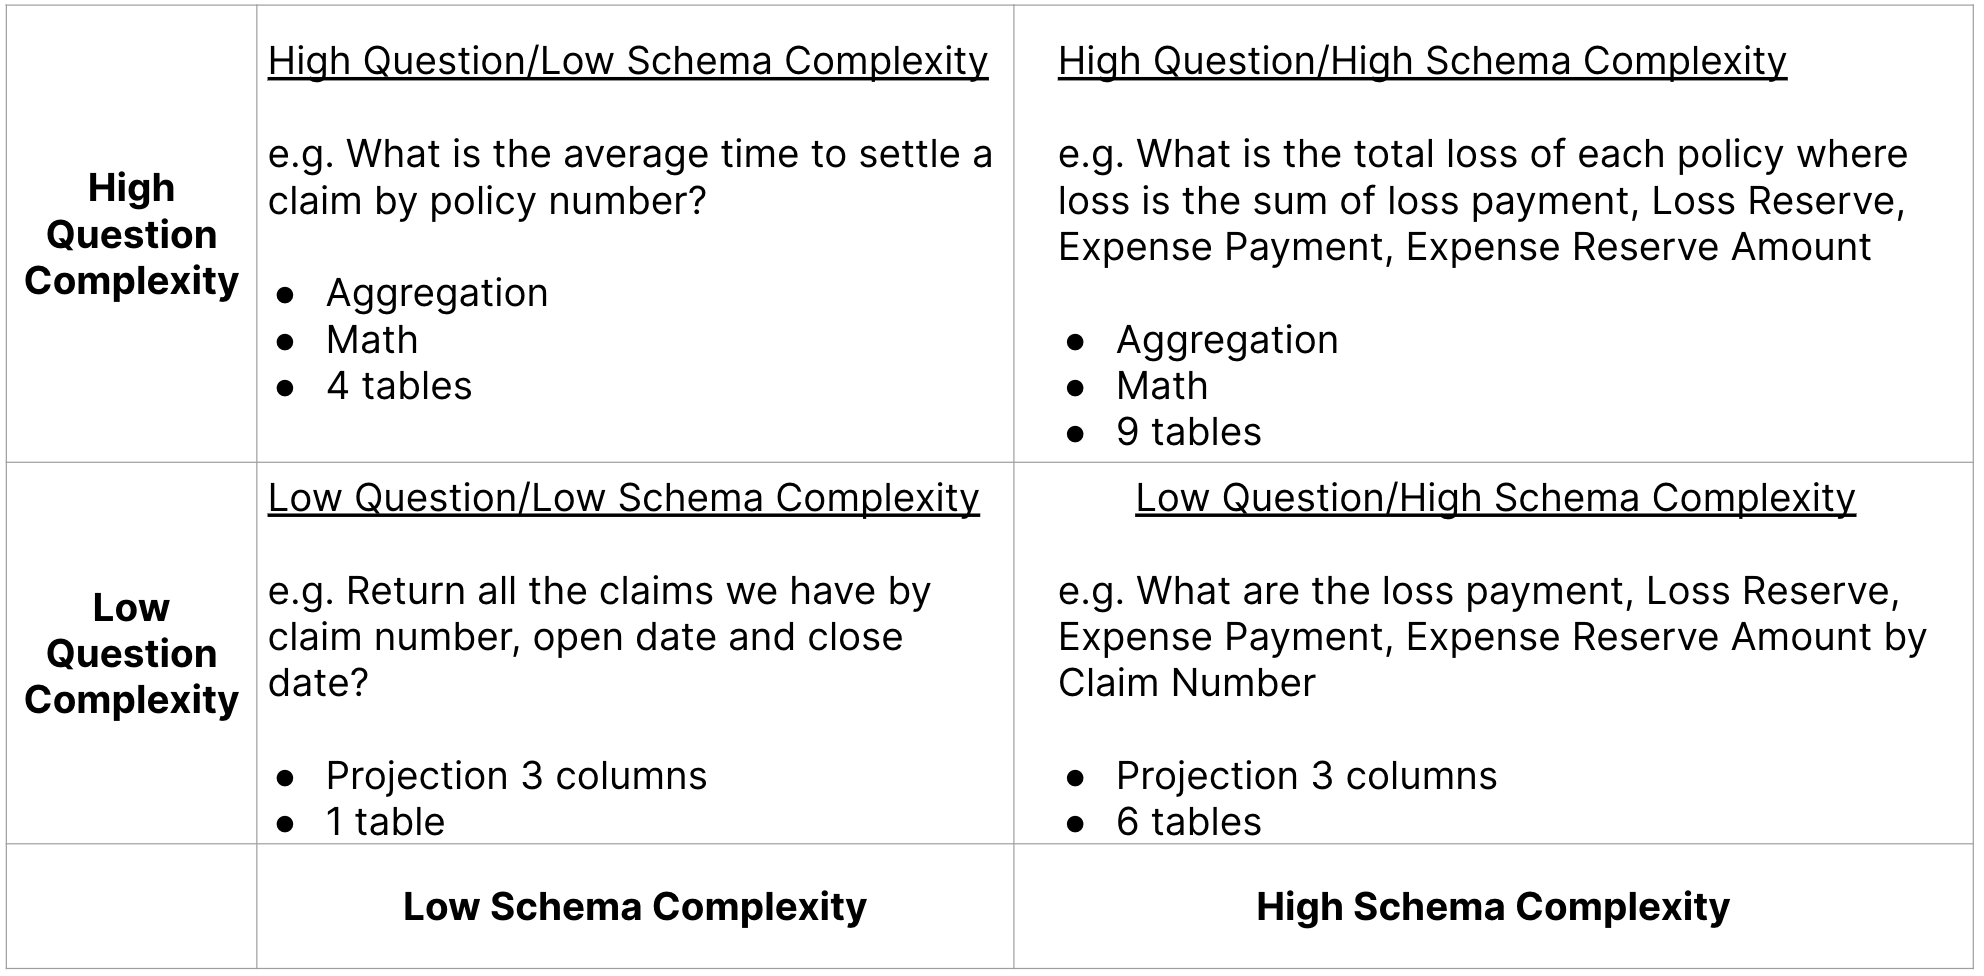
\includegraphics[width=\linewidth]{submissions/Juan2024/results/question_quadrant.png}
\caption{Four quadrants to classify questions: (1) Low Question/Low Schema Complexity, (2) High Question/Low Schema Complexity, (3) Low Question/High Schema Complexity, and (4) High Question/High Schema Complexity}
\label{fig:question_quadrant}
\end{figure}


This 43 questions of the benchmark can be found in \cite{OurPreviousWork} and on 
 Github\footnote{\url{https://github.com/datadotworld/cwd-benchmark-data}}.
While 43 questions may be considered small, the benchmark ensures coverage of key scenarios that reflect real-world enterprise data usage and queries in the insurance domain. 
All the questions in the benchmark are building blocks to answer one of the most important key metrics in the insurance industry: Loss Ratio.
While benchmarks with larger numbers of questions can provide generalizability to evaluate question answering systems and setup leaderboards, the goal of this benchmark is to understand the role of Knowledge Graphs and to what extent the accuracy improves. 
The quadrant provides visibility on the type of extent. 
Furthemore, the question quadrant can be considered as a framework to be applied for other domains; instead of generating a \textit{laundry list} of questions, categorize them in these quadrants. 



\paragraph{Context Layer}
The context layer consists of two parts:
\begin{itemize}
    \item Ontology: Business Concepts, Attributes, and Relationships that describe the insurance domain. 
    \item Mapping: transformation rules from the source SQL schema to the corresponding Business Concepts, Attributes, and Relationships in the target ontology. 
\end{itemize}

For this current version of the benchmark, the context layer is provided in machine readable as RDF: ontology in OWL and mapping in R2RML.
The OWL ontology and R2RML mappings can be used to create the Knowledge Graph either in a virtualized or materialized way. 


\paragraph{Scoring}
The benchmark reports three scores: Execution Accuracy, Overall Execution Accuracy and Average Overall Execution Accuracy.

\begin{itemize}
    \item Execution Accuracy (EA): We follow the metric of Execution Accuracy (EA) from the Spider benchmark \cite{data-spider}. 
An execution is accurate if the result of the query matches the answer for the query. 
Note that the order or the labels of the columns are not taken in account for accuracy.
\item Overall Execution Accuracy (OEA): Given the non-deterministic nature of LLMs, there is no guarantee that given an input question, the generated query will always be the same thus providing the same answer. 
Therefore, every question has a Overall Execution Accuracy (OEA) score which is calculated as (\# of EA)/Total Number of runs. 
\item Average Overall Execution Accuracy (AOEA): The Average Overall Execution Accuracy is the average number of OEA scores for a given set of questions. 
This set could be for all the questions in the benchmark or all the questions in a quadrant. 
\end{itemize}





% As an example, based on this scoring: 
% \begin{itemize}
%     \item 100\% OEA means that every single run generated a query that returned an accurate answer. This means that if there were 100 runs that generated 100 queries, each query returned an accurate result. 
%     \item 50\% OEA means that half of the run returned an accurate answer. This means that if there were 100 runs that generated 100 queries, 50 queries returned an accurate result while 50 queries returned an inaccurate result. 
%     \item 0\% OEA means that every single run generated a query that returned an inaccurate answer. This means that if there were 100 runs that generated 100 queries, each query returned an inaccurate result. 
% \end{itemize}




The benchmark serves as a framework for the results to be reproduced in an enterprise’s own setting using their own enterprise schemas, questions and context. 



% 2) The results of the benchmark. 
% Using GPT-4 and zero-shot prompting, enterprise natural language questions over enterprise SQL databases
% achieved 16.7\% accuracy. 
% This accuracy increased to 54.2\% when a Knowledge Graph representation of the SQL database was used, thus an accuracy improvement of 37.5\%.
% For the questions in each quadrant: 
% \begin{itemize}
%     \item Low Question/Low Schema, knowledge graph accuracy was 71.1\% while the SQL accuracy was 25.5\%
%     \item HighQuestion/Low Schema, knowledge graph accuracy was 66.9\% while the SQL accuracy was 37.4\%
%     \item Low Question/High Schema, knowledge graph accuracy was 35.7\% while the SQL accuracy was 0\%
%     \item High Question/High Schema, knowledge graph accuracy was 38.7\% while the SQL accuracy was 0\%
% \end{itemize}

% The results of the benchmark provide evidence that supports our hypothesis that an LLM powered question answering system that answers a Natural Language question over a Knowledge Graph representation of the SQL database returns more accurate results than a LLM 
% %powered question answering system that answers a Natural Language question over the SQL database 
% without a Knowledge Graph. 

% The main conclusion of this work is that investing in Knowledge Graphs provides higher accuracy for LLM powered question answering systems. 




% The data setup begins with the P\&C Data Model from the OMG as described above. We have made an excerpt of that model to keep the experiment focused, and to allow the questions to be accessible to people who are not experts in the insurance industry.  We express that DDL as a text file. 

% The data itself is expressed  as several tables (CSV format), corresponding to the DDL described above. We have generated sample data for this model, in much the same way as we see in the Spider benchmark\cite{data-spider}.

%The hypothesis we are testing in this experiment is that the performance of a question answering system can be improved when the system includes a knowledge graph representation of the data.  In our experimental setup, we express the knowledge graph as a combination of an ontology that describes the data at a business level, along with mappings from the ontology to the tables in the database.  The ontology is provided to the experimental system as a machine-readable file in OWL, and is shown in a more visual-friendly form in 




% We want to encourage others to perform experiments using the same data. Toward this end, we have published all of  the benchmark data and metadata as a repository in github. 
% The various components in the repository are: 

% \begin{itemize}
%     \item The DDL for the relational database, as a text file.
%     \item The sample data for the tables defined by that DDL.  We publish these in CSV. 
%     \item An OWL file (serialized as RDF Turtle) describing the ontology of the knowledge graph.
%     \item An R2RML file (serialized as RDF Turtle) describing the mappings from the relational schema to the OWL ontology. 
%     \item The questions (natural language) and reference queries (SQL and SPARQL). 
% \end{itemize}

% Wherever possible, we strive to publish these resources in standard formats.  
% The tables themselves are published as CSV, which, while it isn't a standard \textit{per se}, is a format with very broad awareness.  
% The data schema is published as a SQL DDL.  
% There are many dialects of DDL, but most LLMs are conversant in all of them.  
% The knowledge graph context layer components (model and mapping) are published in RDF/TTL, representing OWL and R2RML respectively. 

% In the case of the questions and reference queries, we use SQL or SPARQL for the queries, and English for the questions, but we need a way to represent how they fit together, i.e., which reference queries purport to respond to which questions?  
% For this purpose, we have built a small ontology of questions and queries that describes how we publish these relationships (in RDF/TTL).  
% We also provide a JSON representation of this same information as well. 

% For the purposes of the experiments reported in this paper, these materials were hosted on data.world, as follows: 

% \begin{itemize}
%     \item The DDL is a text file, hosted in data.world as a simple text file.  The data.world API makes this available as is.
%     \item The sample data is hosted in data.world as a set of files. data.world treats text files as tables, and provides a SQL interface to query them. 
%     \item The OWL file is hosted in data.world as a text file, and is available using the same API as the DDL. Additionally, it is synchronized with the gra.fo visualization tool, which allows it to be manipulated in a form that looks like Figure \ref{fig:ontology}.
%     \item The R2RML file is serialized as RDF/TTL, and stored as a file in data.world. By convention, data.world treats any r2rml file as a mapping directive.
%     \item The questions and reference queries are hosted in data.world as queries in a workspace. The \texttt{description} field of the query specifies the natural language text of the query. 
% \end{itemize}

% This setup in data.world provides a number of services that will be helpful as we process the benchmark:

% \begin{itemize}
%     \item The various text files (the OWL ontology and the DDL) are available through the API directly. 
%     \item The sample data stored as multiple CSVs can be queried using SQL directly in the data.world platform (and also through API calls).
%     \item The R2RML file is used to drive semantic virtualization; that is, SPARQL queries that refer to concepts in the OWL ontology are translated by the data.world platform into corresponding SQL queries against the data. 
%     \item The reference queries can be run by hand, to review their results, or through the API by name.  They can also be downloaded through the API, and the text of the queries can be used in contexts outside data.world (e.g., to run on other database systems). 
% \end{itemize}

\subsection{Experimental Setup}


The question answering system we evaluated was a zero-shot prompt to GPT-4, 
%itself, in which a question and some relevant context is provided to an LLM (in this experiment, that was always GPT-4). 
that is instructed to generate a query, which is executed against the database.  
The resulting response is compared to the response given by the reference query. 

The particular parameters to the OpenAI API are as follows: 
\begin{itemize}
    \item max\_tokens = 2048
    \item n = 1
    \item temperature = 0.3
\end{itemize}

Additionally, a timeout was set so that computations that take more than 60 seconds are considered to be failures.

Note that the goal of our experiment is to understand the role of Knowledge Graphs on accuracy.
The focus of the experiment is not to understand how a certain LLM performs with a Knowledge Graph. 
That is why we select only one LLM for our experiment, namely GPT-4. 
Naturally, future work should include a comparison of multiple LLMs in order to understand how a Knowledge Graph can increase accuracy on different LLMs. 


\subsection{Question Answering System for SQL}
The question answering system for SQL is shown in Figure \ref{fig:SQlSystem}.  
The question and the SQL DDL for the database are provided as zero-shot prompt to GPT-4. 
These are combined together using the following simple prompt template:




\noindent \textbf{SQL Zero-shot Prompt}

\fbox{
\begin{minipage}{\linewidth}
\begin{verbatim}
Given the database described by the following DDL: 

INSERT SQL DDL

Write a SQL query that answers the following question. Do not explain the query.  Return just the query, so it can be run verbatim from your response. 

Here's the question: 

INSERT QUESTION
\end{verbatim}
\end{minipage}
}


\noindent We kept the prompt simple for this experiment, because we wanted to focus on the ability of the contextual information (the DDL in the case of SQL) to provide necessary information for the formation of the query. 

The resulting query is sent verbatim to the SQL processor of data.world, which returns an answer in a tabular form.  
This is converted into a Pandas DataFrame for comparison. 
At the same time, the reference query for the question is sent to data.world, and its result is also converted to a DataFrame.  
Once they are both in the form of DataFrames, it is a simple matter to compare them.  
Details of this comparison are available from the Spider project\cite{data-spider}. 





\subsection{Question Answering System for Knowledge Graph}

The question answering system for the Knowledge Graph is shown in Figure \ref{fig:SPARQLSystem}.  
The question and the OWL ontology are provided as zero-shot prompt to GPT-4. 
These are combined together using the following simple prompt template:










\noindent\textbf{SPARQL Zero-shot Prompt}

% \fbox{
% \begin{minipage}{\linewidth}
% \begin{verbatim}
% Given the OWL model described in the following TTL file:

% INSERT OWL ontology

% Write a SPARQL query that answers the question.  The data for your query is available in a SERVICE identified by <{mapped}>.  Do not explain the query.  return just the query, so it can be run verbatim from your response.

% Here's the question: 

% INSERT QUESTION
% \end{verbatim}
% \end{minipage}
% }


As in the SQL case, we kept the prompt simple.  
The extra line about the SERVICE allows the LLM to produce queries that invoke the data.world knowledge graph virtualization layer.  
In principle, this adds some complexity to the SPARQL prompt, but in practice, GPT-4 seemed to handle it very well. 
%This prompt was sent to GPT-4 with the same parameters for the SQL case, including the timeout. 

The resulting query is sent verbatim to the SPARQL processor of data.world, and the result converted to a DataFrame, just as for the SQL case. 

\newpage

\begin{figure}[hbtp]
\centering
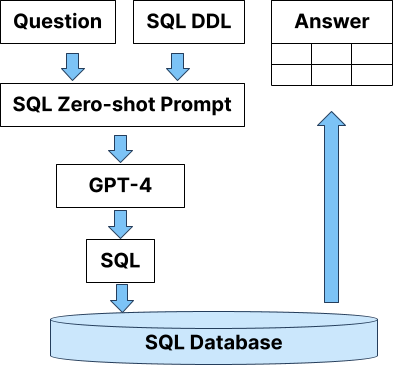
\includegraphics[scale=0.5]{submissions/Juan2024/results/sql_system.png}
\caption{Question Answering System for SQL}
\label{fig:SQlSystem}
\end{figure}


\begin{figure}[hbtp]
\centering
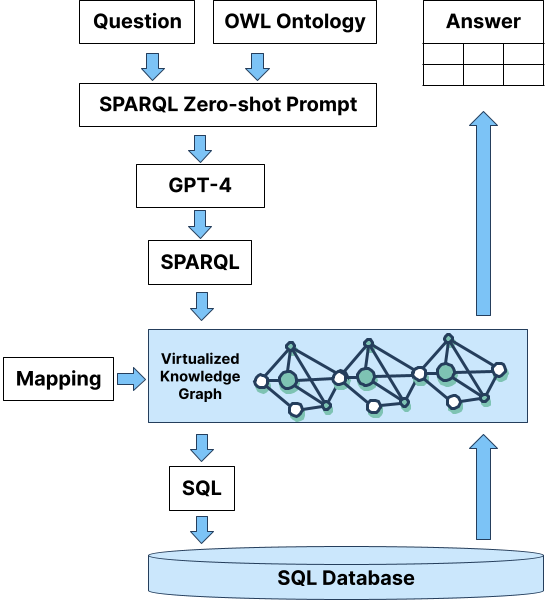
\includegraphics[scale=0.4]{submissions/Juan2024/results/sparql_system.png}
\caption{Question Answering System for Knowledge Graph}
\label{fig:SPARQLSystem}
\end{figure}


\newpage



\subsection{Results}
\label{sec:Results}


The results are presented in four parts 1) overall, 2) question quadrant, 3) partial accuracy and 4) inaccurate results. 
In the results, we refer to
\begin{itemize}
    \item SPARQL as question over Knowledge Graph representation of the SQL database and 
    \item SQL as questions directly on the SQL databases without a Knowledge Graph.
\end{itemize}


Given that the OEA of a question is a percentage, the results are presented as a heatmap. 
Every cell corresponds to a generated query for the given question. The value in the cell is the OEA for that question. 
The green color corresponds to 100\% OEA. The red color corresponds to 0\% OEA. The color scale goes from green to red.

The Overall and Quadrant results are presented in Table \ref{table:Results}.

\subsubsection{Overall}
By grouping all the questions in the benchmark, SQL achieves an AOEA of 16.7\%. 
In comparison, SPARQL achieves an average OEA of 54.2\% as shown in Figure \ref{fig:fig1}. 
The heatmap that depicts the OEA for each question is shown in Figure \ref{fig:fig2}:
Therefore, overall SPARQL accuracy was 3x the SQL accuracy.

Overall, Natural Language questions translated to SPARQL over a Knowledge Graph representation of the SQL database achieved 3x the accuracy of natural language questions translated to SQL and executed directly over the SQL database. 
Combining all the questions into one overall result is not satisfactory because there are nuances to the types of questions. 
This is why we also present the results in each of the quadrants.



\begin{wrapfigure}{r}{0.5\textwidth}
  \begin{center}
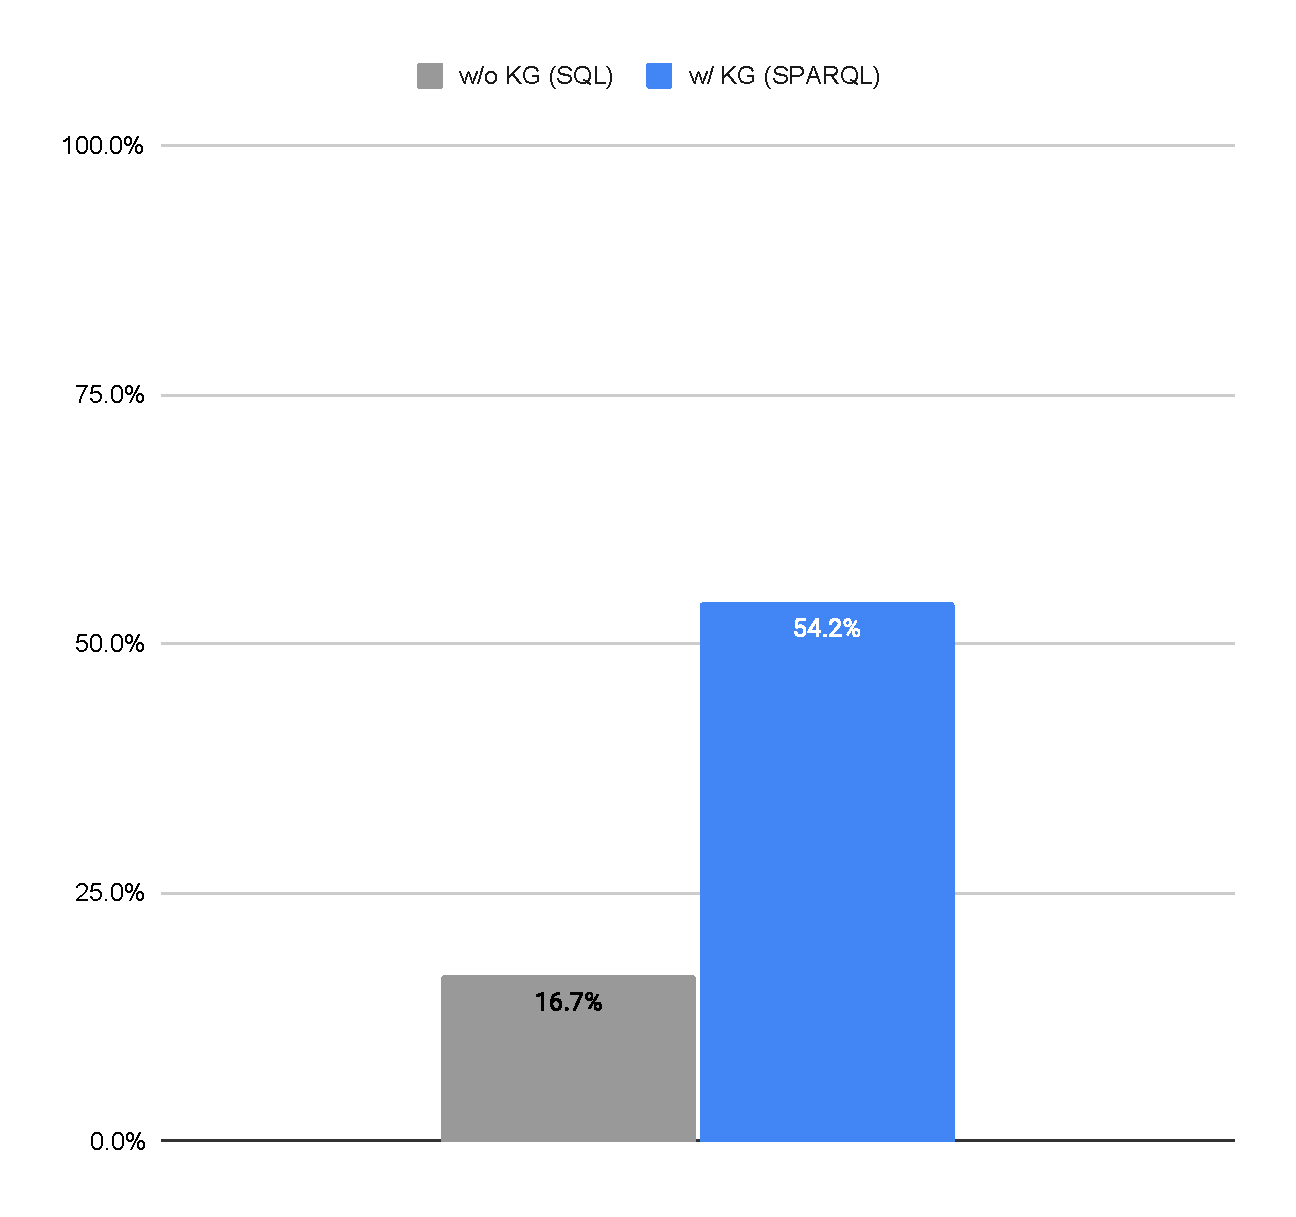
\includegraphics[scale=0.3]{submissions/Juan2024/results/overall.pdf}
\caption{Average Overall Execution Accuracy (AOEA) of SPARQL and SQL for all the questions in the benchmark}
\label{fig:fig1}
\end{center}
\vspace{-2cm}
\end{wrapfigure}

\subsubsection{Quadrant}

Figure \ref{fig:fig3} presents the AOEA scores for questions in each quadrant. 
Figure \ref{fig:fig4} presents the heat map for each quadrant.
We observe the following results: 
\begin{itemize}
    \item Low Question/Low Schema: SQL achieves an AOEA of 25.5\%. In comparison, SPARQL achieves an AOEA of 71.1\%. The SPARQL accuracy is 2.8X the SQL accuracy.

    \item High Question/Low Schema: SQL achieves an AOEA of 37.4\%. In comparison, SPARQL achieves an AOEA of 66.9\%. The SPARQL accuracy is 1.8X the SQL accuracy.

    \item Low Question/High Schema: SQL was not able to answer any question accurately. In comparison, SPARQL achieves an AOEA of 35.7\%.

    \item High Question/High Schema: SQL was not able to answer any question accurately. In comparison, SPARQL achieves an AOEA of 38.7\%.

\end{itemize}

Per the hypothesis, SPARQL achieves higher accuracy than SQL in every quadrant. 
Furthermore, it is surprising to observe that SQL was not able to answer any question in the High Schema Complexity quadrants. 
These results by quadrant sheds further light on understanding the extent. 
In each quadrant, SPARQL accuracy is higher than the SQL accuracy. 
While the SPARQL accuracy is 2.8X the SQL accuracy for Low Question/Low Schema and 1.8X for High Question/Low Schema, it was unforeseen that SQL was not able to accurately answer any questions for Low Question/High Schema and High Question/High Schema. 
The results also lead us to understand when SQL starts to fail.
When a question requires more than 4 tables to provide then answer, the accuracy drops to zero. 

\renewcommand{\arraystretch}{1.2}
\begin{table}[h!]
\centering
\begin{tabular}{|l|c|c|c|}
\hline
\ & \textbf{w/o KG (SQL)} & \textbf{w/ KG (SPARQL)} & \textbf{Improvement}\\
\hline
\textbf{All Questions} & 16.7\% & 54.2\% & 37.5\%\\
\hline
\textbf{Low Question/Low Schema} & 25.5\% & 71.1\% & 45.6\%\\
\hline
\textbf{High Question/Low Schema} & 37.4\% & 66.9\% & 29.5\%\\ 
\hline
\textbf{Low Question/High Schema} & 0\% & 35.7\% & 35.7\%\\
\hline
\textbf{High Question/High Schema} & 0\% & 38.5\% & 38.5\%\\
\hline
\end{tabular}
\caption{Average Overall Execution Accuracy (AOEA) of Overall and Quadrant Results}
\label{table:Results}
\end{table}















\begin{figure}
% \begin{wrapfigure}{R}{0.5\textwidth}
  \begin{center}
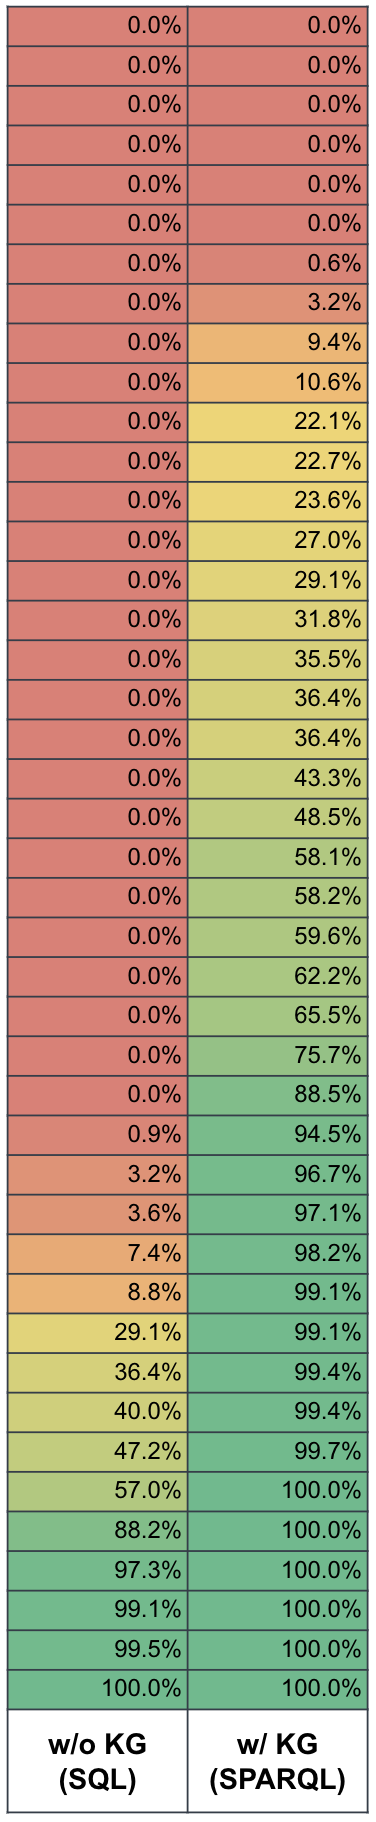
\includegraphics[scale=0.5]{submissions/Juan2024/results/overall_heatmap.png}
\caption{Overall Execution Accuracy (OEA) of SPARQL and SQL for all the questions as a heatmap}
\label{fig:fig2}
\end{center}
% \vspace{-4.3cm}
% \end{wrapfigure}
\end{figure}


\begin{figure}[hbtp]
\centering
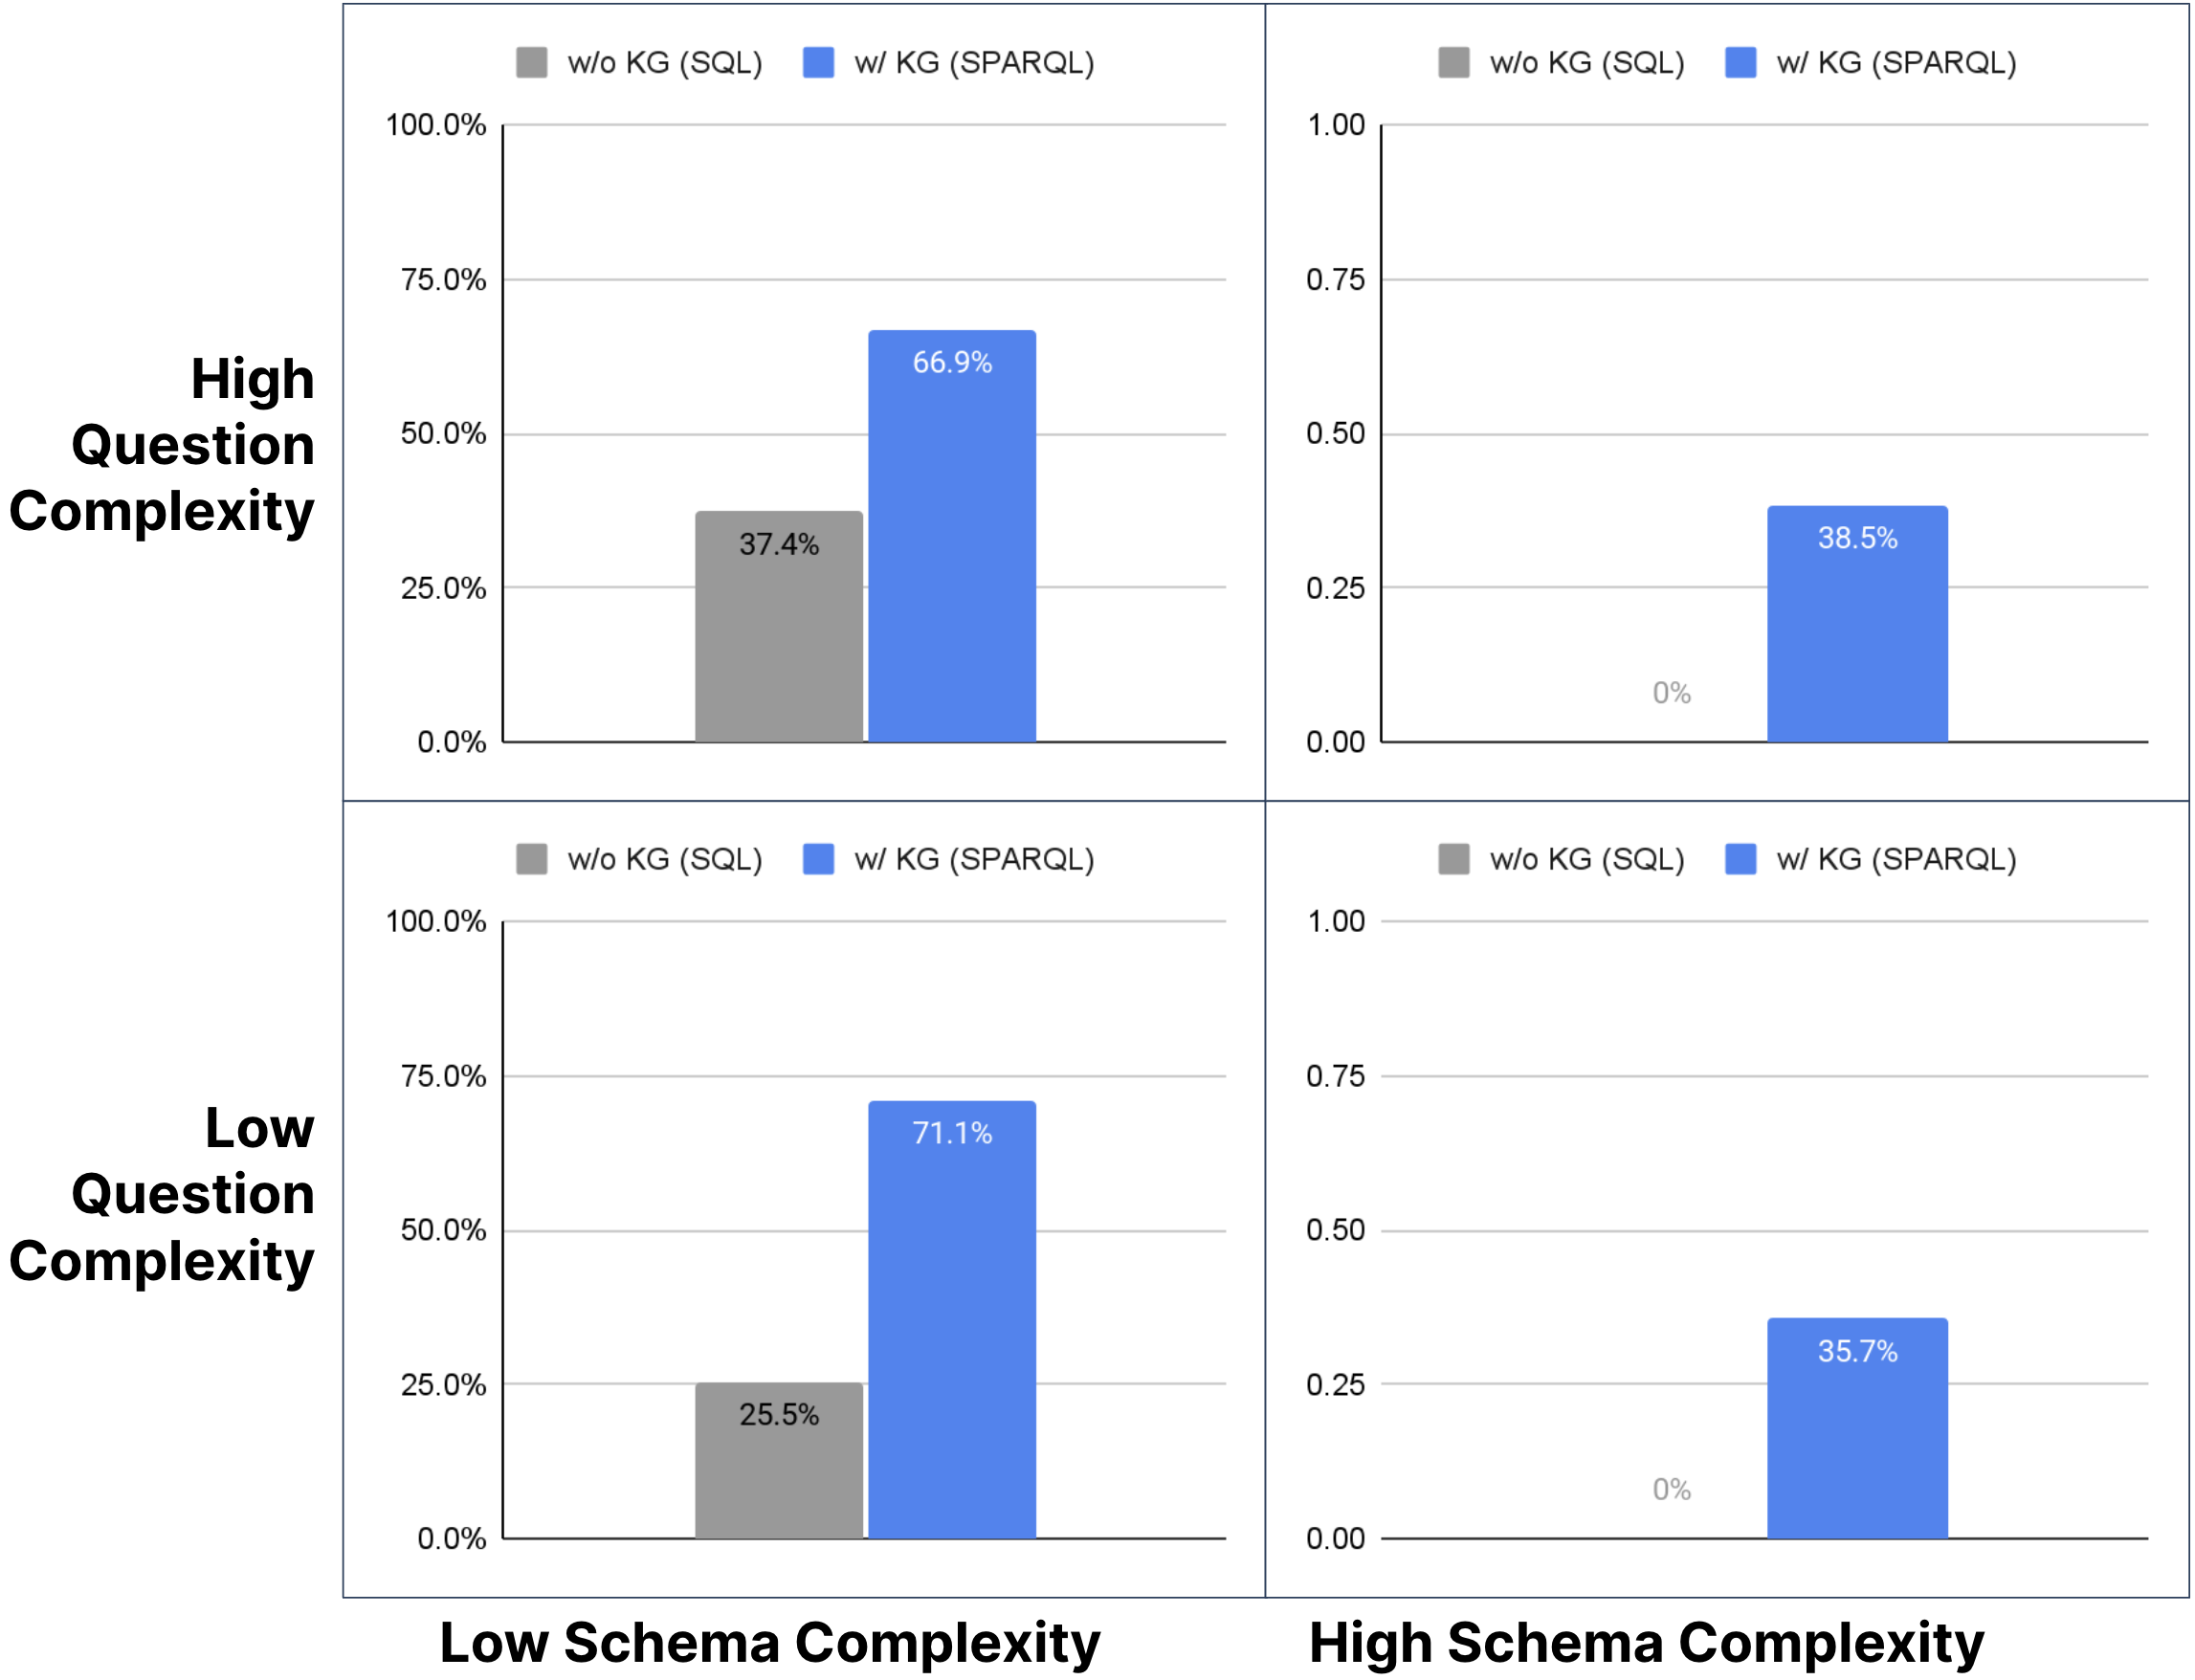
\includegraphics[scale=0.35]{submissions/Juan2024/results/quadrant.png}
\caption{Average Overall Execution Accuracy (AOEA) of SPARQL and SQL for each quadrant}
\label{fig:fig3}
\end{figure}




\begin{figure}[hbtp]
\centering
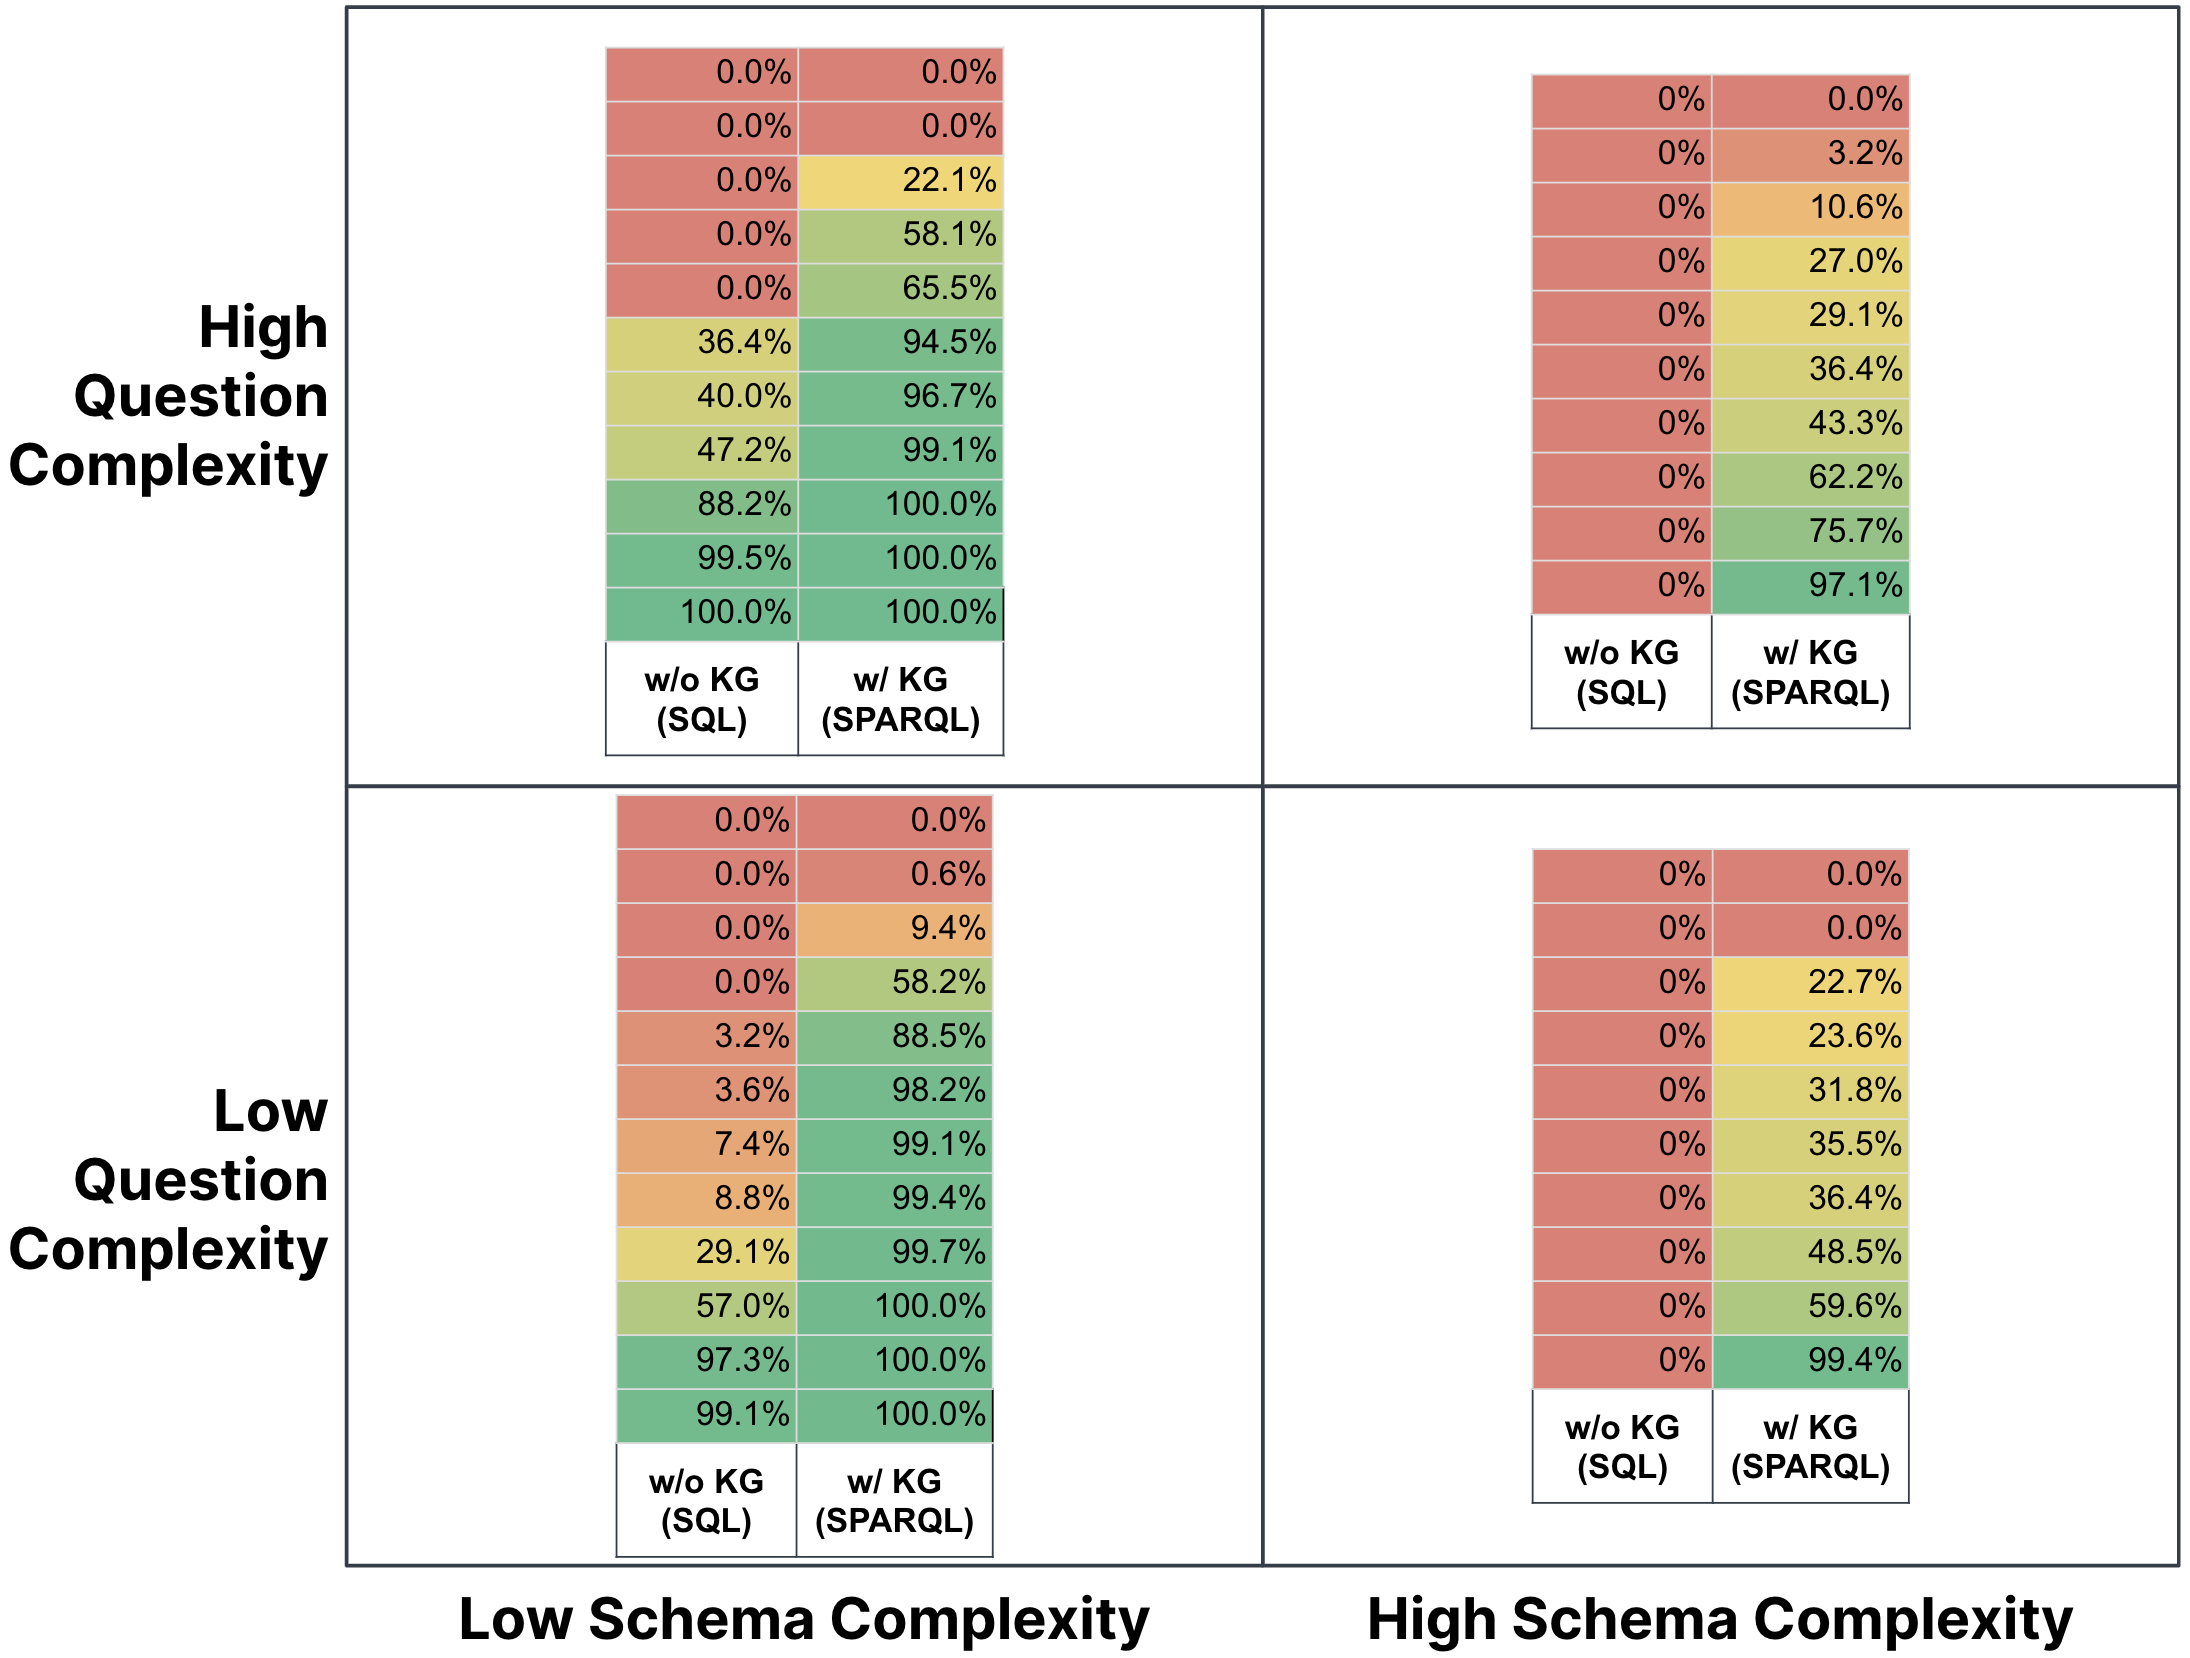
\includegraphics[scale=0.35]{submissions/Juan2024/results/quadrant_heatmap.png}
\caption{Overall Execution Accuracy (OEA) of SPARQL and SQL for each quadrant as a heatmap}
\label{fig:fig4}
\end{figure}






\subsubsection{Partial Accuracy}

We manually analyzed the generated SQL and SPARQL queries and observed that a subset of queries produced partially accurate results.
We consider a partially accurate answer to be one where the returned answers are accurate but incomplete. 
During the manual analysis, the following patterns for partially accurate answers are observed: 

\begin{itemize}
    \item \textbf{Overlap:} the columns returned by the query are correct, however, they are  a subset of the accurate answer. In some cases, they include other columns that are not part of the expected answer. This can be seen as a form of a semantic overlap\cite{DBLP:conf/dexa/GodfreyG99}. 
    \item \textbf{Return Identifier:} An internal identifier was returned instead of the appropriate label.   
\end{itemize}

Consider the question \textit{Return all the claims we have by claim number, open date and close date?} and the following generated SQL and SPARQL query: 

\textbf{SQL}
\begin{verbatim}
SELECT Claim_Identifier, Claim_Open_Date, Claim_Close_Date
FROM Claim
\end{verbatim}

\textbf{SPARQL}
\begin{verbatim}
SELECT ?claim ?claimOpenDate ?claimCloseDate
WHERE {
    ?claim a in:Claim ;
           in:claimNumber ?claimNumber ;
           in:claimOpenDate ?claimOpenDate ;
           in:claimCloseDate ?claimCloseDate .
}
\end{verbatim}

The answer for claim open date and claim close date are accurate and is a subset of the correct answer. 
However in the SQL query, the \texttt{Claim\_Identifier} column is being returned as the claim number, when in fact, the claim number is actually the column \texttt{company\_claim\_number}. 
In the SPARQL query case, the variable \texttt{?claim} is returned which binds to the IRI that uniquely identifies each claim. 
The claim number is not returned.

% Another issue we observed is that for a question that involved determining the average days between two dates, the generated SQL and SPARQL were both  semantically correct but the reason the query did not execute was due to a syntax error on date diff.
%For a query with incorrect syntax, the model could be fine tuned or the query could be fixed in a post processing phase. 

In practice, if a user is interacting with a system and the results are missing a column, they could ask for the missing column or provide a label instead of an identifier. 
Therefore partial accuracy may be acceptable for users. 
However this is an open question on how to define partial accuracy and how to score it.
%Finally, this version of the benchmark did not include functions or operations over dates (see Section \ref{sec:ResearchAgenda} for a discussion on next steps on this topic).

\subsubsection{Inaccuracy}

During the manual analysis of the generated queries, we also observed query characteristics that generated the inaccurate answers. 
These characteristics were different for SQL and SPARQL. 

\paragraph{SQL Inaccuracy}
The following three types of inaccuracies were observed: 
\begin{itemize}
    \item \textbf{Column Name Hallucinations}: Column names were generated that do not exist in the corresponding table. 
    \item \textbf{Value Hallucinations}: Generated value applied as a filter on a column where that value does not exist in the database.
    \item \textbf{Join Hallucinations}: Generated joins that are not accurate. 
\end{itemize}

%[NEED EXAMPLE:] Consider the following SQL query: 
\paragraph{SPARQL Inaccuracy}

\begin{itemize}
    \item \textbf{Incorrect Path:} The generated query does not follow the correct path of the properties in the ontology. The generated path goes from A to C when the correct path is A to B to C. 
    \item \textbf{Incorrect Direction:} The generated query swaps the direction of a property. The generated direction is B to A, when the correct direction is A to B. 
\end{itemize}

%[NEED EXAMPLE:] Consider the following SPARQL query: 

The inaccuracy of SQL queries are based on hallucination while the inaccuracy of SPARQL queries are based on path inconsistency. 
The SQL hallucinations are evident: column names that don’t exist in a table and values that the LLM does not know if they exist in the data.
The joins may seem plausible, but they are not how the database was designed, thus returning empty results. 
For SPARQL queries, the generated paths are indicative that the LLM knew what the correct starting and end node was and the error was on defining the correct path from the start node to the end node. 
One could even argue that the LLM appears to do some sort of reasoning but not always getting it correct.
This observation is what led us to the second part of our work. 

% To our surprise, while manually analyzing the generated SPARQL queries, we did not observe a hallucinated class or property. 
% Anecdotally, we have observed that when a user goes to ChatGPT and asks a similar prompt, it does hallucinate properties in SPARQL query.
% It is unclear why it did not hallucinate in the benchmark results. 
% A speculation is that the prompt specifically stated \textit{return just the query, so it can be run verbatim from your response.} and this avoided hallucinations. 
% However, the prompt structure is the same for SQL and SPARQL so the question remains, why did it hallucinate in SQL and not in SPARQL. 
% See Section \ref{sec:ResearchAgenda} for further discussion on next steps. 

\section{Ontologies to the Rescue}

Consider the following knowledge represented in an ontology of a knowledge graph: \textit{a Policy is sold by an Agent}. 
If an LLM generated SPARQL query representing the statement \textit{an Agent is sold by a Policy}, it would be inconsistent because it does not match the semantics of the ontology (i.e. this doesn't make sense). 
Our intuition is two-fold. 
First, by leveraging the ontology of knowledge graph, we can check the LLM generated SPARQL query and detect these types of errors. 
Second, we can also use the LLM to repair incorrect SPARQL queries.

For example, assume the following question \textit{``return all the policies that an agent sold"}, resulted in the following SPARQL query:


%\begin{lstlisting}[language=SPARQL]
\begin{verbatim}
SELECT ?agent ?policy
WHERE {
  ?agent :soldByAgent ?policy . 
  ?agent rdf:type :Agent 
}
\end{verbatim}
%\end{lstlisting}

\noindent and given the following snippet of an OWL ontology

\begin{verbatim}
:soldByAgent a owl:DatatypeProperty;
  rdfs:domain :Policy ;
  rdfs:range :Agent .
\end{verbatim}

\noindent we could determine that the generated query should be correct if the domain of \texttt{:soldByAgent} is \texttt{:Policy}.
However, per the query, the domain is \texttt{:Agent} and assuming they are disjoint, the generated query does not match the semantics of the ontology, thus it is incorrect. 
Given an explaination of this error, we could then prompt the LLM to try again.

We investigate the following research questions:

\noindent \textbf{RQ3}: To what extent can the accuracy increase by leveraging the ontology of a knowledge graph to detect errors of a SPARQL query and an LLM to repair the errors?
    
\noindent \textbf{RQ4}: What types of errors are most commonly presented in SPARQL queries generated by an LLM?

The hypothesis is the following: \textit{An ontology can increase the accuracy of an LLM powered question answering system that answers a natural language question over a knowledge graph.}

This first part of our approach is the \textbf{Ontology-based Query Check} (OBQC), which checks if the query is valid by applying rules based on the semantics of the ontology. 
A set of rules checks the semantics of the body of the query (i.e. the WHERE clause).
Another set of rules checks the head of query (i.e. the SELECT clause). 
It is important to clarify that the Ontology-based Query Check does not use an LLM. 
It is a deterministic rule-based approach based solely on the semantics of the ontology. 
If the OBQC detects an error, we could try to repair the query.

Repairing databases\cite{10.1145/1514894.1514899} and programs\cite{10.1145/3318162,10.1145/3631974} has been an long standing research area in computer science. 
Recently, LLMs have been applied to repair programs\cite{bouzenia2024repairagent, 10.1145/3611643.3613892}.
Inspired by these approaches, consider the following example. 
Once a SPARQL query is detected to be incorrect, we can define an explanation for the reason why it is incorrect. 
Per our running example, an explanation is the following: \textit{The property
:soldByAgent has domain :Policy, but its subject ?agent is a :Agent, which isn’t a subclass of :Policy.}.
What if we can pass the incorrect SPARQL query, with this explanation and prompt the LLM to rewrite the query? 

The second part of our approach is \textbf{LLM Repair}, which repairs the SPARQL query generated by the LLM. 
It takes as input the incorrect query and the explanation coming from the rule(s) that was fired as an explanation to why the query is incorrect and re-prompts the LLM. 
The result is a new query which can then be passed back to the OBQC. 
Our approach gives us the opportunity to understand the capability of an LLM to repair a SPARQL query and thus further improve the accuracy.
Figure \ref{fig:overview} depicts the overview of our approach. 

\begin{figure}[hbtp]
\centering
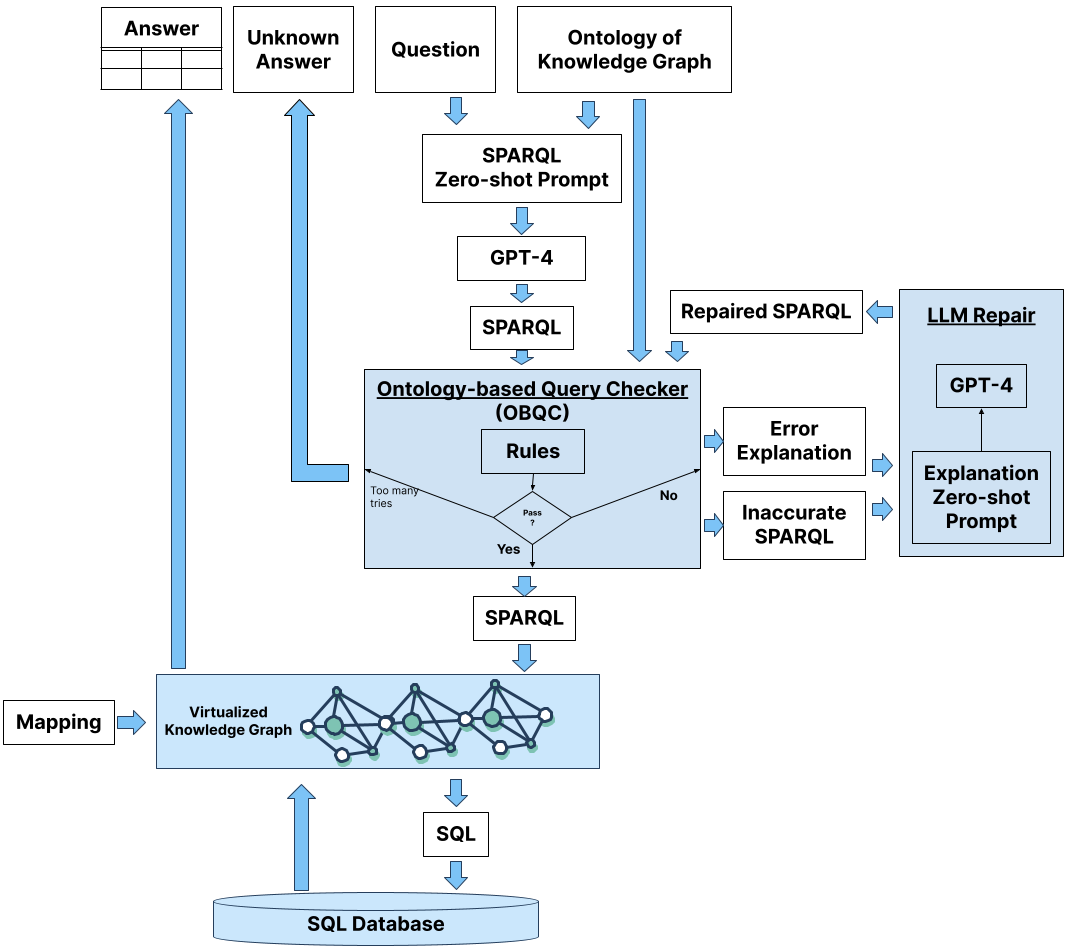
\includegraphics[scale=0.4]{submissions/Juan2024/images/Overview.png}
\caption{Overview of our Ontology-based Query Checker and LLM Repair approach}
\label{fig:overview}
\end{figure}

% We evaluated our approach using the benchmark from our first contribution and our primary findings are the following: 
% \begin{itemize}
%     \item By grouping all the questions in the benchmark, the OBQC and LLM Repair increased the accuracy 72.55\%. If the repairs were not successful after three iterations, an unknown result was returned, which occurred 8\% of the time. The result is an error rate of 20\%. 
%     \item Low complex questions on low complex schemas achieves an error rate of 10.46\%, which is arguably at levels deemed to be acceptable by users. 
%     \item All questions on high complex schemas substantially increased the accuracy. 
%     \item The rules related to the body of the query domain were invoked 70\% of the time while the rules related to the head of the query were invoked 30\% of the time. 
% \end{itemize}

% Comparing these results to our previous work \cite{OurPreviousWork}, we see a progression towards higher accuracy and reduced error rate. 

% Previously, we showed that by using GPT-4 and zero-shot prompting, enterprise natural language questions over
% enterprise SQL databases achieved 16.7\% accuracy.
% This accuracy increased to 54.2\% when a Knowledge Graph
% representation of the SQL database was used.
% Thus an 3x accuracy improvement (37.5\%). 
% By using the same zero-shot prompting on GPT-4 and adding \textbf{Ontology-Based Query Check} and \textbf{LLM Repair}, that new accuracy is 72.55\%.
% That is over a 4x accuracy improvement compared to not using a knowledge graph at all. 

% If we look at the error rate, we also see a substantial decrease. 
% Without leveraging a knowledge graph, the error rate is 83.3\%.
% The error rate decreased to 45.8\% when using a knowledge graph.
% Given that we consider an unknown result in our approach because the \textbf{LLM Repair} is not able to repair and the \textbf{Ontology-Based Query Check} catches the error, the error rate has been further decreased to 19.44\%. 

% The main conclusion is that we provide further strong evidence that investing in semantics, ontologies and knowledge graphs are prerequisites to achieve higher accuracy for LLM-powered question answering systems. 


% \subsection{Research Question and Hypothesis}
% Our research goal is to understand how to increase the accuracy of Large Language Models powered question answering systems. 
% By continuing to leverage knowledge graphs, our intuition is that the ontology can be used to detect errors in queries and an LLM be used to repair the query, thus improving the accuracy. 
% Specifically, this intuition is based on the observation of our previous work \cite{OurPreviousWork}: the LLM generated a SPARQL query that produced inaccurate results due to the following: 
% \begin{itemize}
%     \item Incorrect Path: The generated query did not follow the correct path of the properties in the ontology. The generated path goes from A to C when the correct path is A to B to C. 
%     \item Incorrect Direction: The generated query swaps the direction of a property. The generated direction is B to A, when the correct direction is A to B.
% \end{itemize}

% Therefore, 



\subsection{Ontology-based Query Check}
Knowledge Graphs defined using the Semantic Web technology stack (specifically, RDF, RDFS, OWL and SPARQL) have been built on a rigorous logical foundation. 
The exact meaning of a statement (triple) in RDF is given in terms of predicate logic; the meaning of a model in RDFS or OWL is specified according to a logical foundation \cite{10.1145/3382097,DBLP:journals/csur/HoganBCdMGKGNNN21,DBLP:series/synthesis/2021Hogan}\footnote{For an introduction to knowledge graphs and semantic web technologies, we refer the reader to the textbooks ``Semantic Web for the Working Ontologist" and ``Knowledge Graphs" \url{https://kgbook.org/} }. 
The meaning of a SPARQL query is specified in terms of these logical foundations. 
A practical upshot of this theoretical framework is that it is possible to know exactly what constraints a model in RDFS or OWL places on the correctness of a SPARQL query, and these constraints can be described in an executable way in SPARQL. 
%We leverage this foundation to create an ontology-based query check system for SPARQL queries. 
The approach takes two inputs: a SPARQL query and an ontology. 
The output consists of a list of sentences that describe ways in which the SPARQL query deviates from the specifications in the ontology. 

The check system relies on the declarative nature of SPARQL, the structure of Basic Graph Patterns and, the ability to query the ontology via SPARQL itself. 
If the generated query deviates from the ontology, the approach outlines how.
The approach to achieve this is threefold:

First, a SPARQL query consists of a pattern to be matched against the data (specified after the keyword WHERE in the query); known as a Basic Graph Pattern (BGP) of the query. 
The process begins with extraction of BGPs from the generated SPARQL query, replacing variables with resources from a reserved namespace (prefixed with qq:). Some portions of the original query logic, including the SELECT clause, subquery structures, filters, UNIONs, OPTIONAL and NOT clauses, aren't considered since the focus is on examining the compatibility of the BGP with the ontology structure. We leave that for future work. 
However, note that violations of BGPs in an OPTIONAL or FILTER NOT EXISTS / MINUS context are not ignored as they can also provide vital insights into the query understanding.

Second, a \textit{conjunctive graph}\footnote{using RDFLib nomenclature} is constructed by encapsulating two named graphs: \texttt{:query} and \texttt{:ontology}, representing the SPARQL query's BGP-turned-RDF and the ontology, respectively.

Third, the ontology consistency rules are applied guided by the formal logic of RDFS and OWL. The rules are implemented in SPARQL which query the \texttt{:query} and \texttt{:ontology} graphs and identify instances where the query diverges from the ontology.

Note that this ontology-based query check approach could be extended to other Knowledge Graphs that lack a rigorous semantic foundation, such as property graphs. 
However, property graphs do not have well-defined standardized schema language and an inference system. 
This would need to be explicitly defined in order for our approach to be applied.



\subsubsection{Rules}
We defined two set of rules based on the body and the head of a query. 
The body rules check that the Basic Graph Patterns of a SPARQL query (i.e. WHERE clause) matches the semantics of an ontology. 
Our approach follows a subset of the RDF Schema (RDFS) semantics\footnote{\url{https://www.w3.org/TR/rdf11-schema/}}. 
The body rules are: 
\begin{itemize}
    \item Domain: If the domain of a property p is a class C, then the subject of any triple using p as a predicate must be a member of class C.
    \item Range: If the range of a property p is a class C, then the object of any triple using p as a predicate must be a member of class C.
    \item Double Range: If two triples make conflicting requirements on the range of a property then error. 
    \item Double Domain: If two triples make conflicting requirements on the domain of a property then error
    \item Domain Range: If the object of a first triple is the subject of a second triple, then the range of the property of the first triple should be the same as the domain of the property of the second triple.
    \item Incorrect Property: All the properties in the query need to exist in the ontology. 

\end{itemize}

The head rules check the head of a SPARQL query (i.e. SELECT clause). 
A common error for an LLM is to include extra values in the SELECT clause or to leave some out. 
These errors have nothing to do with the ontology. 
However, a very common error is to include a variable in the SELECT clause that will be bound to an IRI (an identifier).
The head rules are:
\begin{itemize}
    \item Subject Output: if a query selects a variable that is the subject of a basic triple pattern, then it is an IRI.
\item IRI Output: if a predicate has a specified range which is a class, then the object of that triple is an IRI.
\end{itemize}

For simplicity, in this paper we only provide an example of the Domain Rule. The description of the implementation for all the rules can be found in \cite{SecondContribution,DBLP:journals/corr/abs-2405-11706}.

The Domain rule (rdfs:domain in RDF Schema) is defined in English as follows: 
If the domain of a property p is a class C, then the subject of any triple using p as a predicate must be a member of class C.
The domain rule is formally defined as: 
\begin{verbatim}
IF 
    ?p rdfs:domain ?C . 
    ?s ?p ?o .  
THEN 
    ?s rdf:type ?C .
\end{verbatim}

The following SPARQL query is a representation of this domain rule which detects a violation: 
\begin{lstlisting}[language=SPARQL]
SELECT ?p ?domain ?s ?class WHERE {
    GRAPH :query{
      ?s ?p ?o .
      ?s a ?class .
    }
    GRAPH :ontology{
      ?p rdfs:domain ?domain.
      FILTER (ISIRI (?domain))
    }
    FILTER NOT EXISTS {
        ?class rdfs:subClassOf* ?domain .
    }
}
\end{lstlisting}


The following example shows how the domain rule is used to check a BGP against an ontology.
Suppose the LLM generated the following query: 

\begin{lstlisting}[language=SPARQL]
SELECT ?agent WHERE {
  ?agent :soldByAgent ?policy . 
  ?agent rdf:type :Agent 
}
\end{lstlisting}

This query has a BGP consisting of two-triples: 

\begin{verbatim}
 ?agent :soldByAgent ?policy . 
 ?agent rdf:type :Agent

\end{verbatim}

The BGP is turned into RDF graph by replacing the variables with resources from a reserved namespace (prefixed with qq:): 

\begin{verbatim}
  qq:agent :soldByAgent qq:policy . 
  qq:agent rdf:type :Agent
\end{verbatim}

Now, suppose the ontology includes the following definition of \texttt{:soldByAgent}: 

\begin{verbatim}
:soldByAgent 
  rdfs:domain :Policy ;
  rdfs:range :Agent .
\end{verbatim}

The conjunctive graph in nquads is the following: 

\begin{verbatim}
:query {
    qq:agent :soldByAgent qq:policy . 
    qq:agent rdf:type :Agent  .
 }
:ontology {
    :soldByAgent 
      rdfs:domain :Policy ;
      rdfs:range :Agent . 
}
\end{verbatim}


The first clause, on the graph \texttt{:query}, finds the precondition for \texttt{rdfs:domain}; there is a triple with predicate \texttt(?p) whose subject is a member of some \texttt{class}.
The second clause searches the ontology for a relevant domain definition; that is, that same property \texttt{?p} has a specified domain.  This query ignores domain definitions that are not IRIs, which would typically include domains that are UNIONs or INTERSECTIONs of other classes. We have simplified the query for exposition in this paper, but it would be easy enough to extend the query to deal with other OWL constructs. We leave this as future work.
Finally, the FILTER clause of this query checks to make sure that the class specified in the  input query (\texttt{?class}) is not included in the domain (\texttt{?domain}). 
If all of these conditions in the evaluation query hold, then we have found a violation of the ontology in the query.  

Continuing our example, in the \texttt{:query} graph, we have a match for the first clause, with the binding 

\begin{verbatim}
?s -> qq:agent
?p -> :soldByAgent
?class -> :Agent
\end{verbatim}

The second clause searches \texttt{:ontology} for a triple matching

\begin{verbatim}
?soldByAgent rdfs:domain ?domain 
\end{verbatim}

this matches, with \texttt{?domain} bound to \texttt{:Policy} (which is indeed an IRI). 
Finally, we test whether 

\begin{verbatim}
:Agent rdfs:subClassOf* :Policy .
\end{verbatim}

Notice that the meaning of the * in SPARQL implies that this would succeed if :Agent were the same as :Policy.  
But in this case, they are not the same, and there is no such triple, so the FILTER NOT EXISTS condition succeeds, and the check comes up with a match, with the following bindings 

\begin{verbatim}
?p -> :soldByAgent
?domain -> :Policy
?s -> qq:agent
?class -> :Agent
\end{verbatim}

This information is not very understandable to a human, and might not be usable to an LLM.  
But it can be formatted into a meaningful sentence in English as follows: 

The property \texttt{:soldByAgent} has domain \texttt{:Policy}, but its subject \texttt{?agent} is a \texttt{:Agent}, which isn't a subclass of \texttt{:Policy}.

For each check rule, we provide a template that can create this explanation.  In this case, the template is:
\textit{The property \{p\} has domain \{dom\}, but its subject \{s\} is a \{class\}, which isn't a subclass of \{dom\}}



\subsection{LLM Repair}
The LLM Repair is a prompt that takes as two inputs: 1) the list of issues for which the query is incorrect which is the output of the OBQC and 2) the incorrect SPARQL query. 
The prompt is the following:

\noindent\textbf{Explanation Zero-shot Prompt}

% \fbox{
% \begin{minipage}{\linewidth}
% \begin{verbatim}

% We have a query 

% INSERT QUERY 

% with some issues outlined here 

% INSERT ISSUES 

% Please re-write it.
% \end{verbatim}
% \end{minipage}
% }



The output is a new LLM generated SPARQL query, which is passed again to the OBQC.
This cycle repeats until the check pass, or an upper limit of cycles is reached. 
In our experiments, the limit is 3. 
In this latter case, the query generation is said to be unknown; there is no point in sending a query that is known to be faulty to the database. 

It is instructive to note that the LLM repair focuses on that task; we do not repeat the question nor the ontology to the LLM. 
The ontology input was taken into consideration by the OBQC, and the question is reflected in the query so far. 

It is also noteworthy that there are two possible outcomes; we can achieve a query that we have considerable confidence in (because it matches the semantics of the ontology), or we fail to create such a query. 
In the latter case, we are aware of the failure of the system. 
In contrast to a pure LLM-based system which is prone to \textit{hallucinations}, when we get the wrong answer, we know it, and can report that to the user. 


\subsection{Results}
% The experiments reported here use the same data as the Chat with the Data benchmark from our previous work, which is available on github\footnote{\url{https://github.com/datadotworld/cwd-benchmark-data}}.
The results consider three cases: 1) accurate queries (that get the right answer), 2) inaccurate queries (that get the wrong answer), and 3) {\it unknown} queries, queries that we know are incorrect and are not able to repair. 
As we summarize the results, we follow the metric of Execution Accuracy (EA) from the Spider benchmark \cite{data-spider}.
% An execution is accurate if the result of the query matches the answer for the query. 
% Note that the order or the labels of the columns are not taken in account for accuracy. 

We report the following metrics for a SPARQL query generated by an LLM: 

\begin{itemize}
    \item Execution Accuracy First Time: if the OBQC returns true the first time which results in an accurate execution.
    \item Execution Accuracy with Repairs: if the OBQC returns false the first time and the LLM Repair results in an accurate execution. 
    \item Execution Unknown with Repairs: if the OBQC returns false the first time and the LLM Repair is unable to repair after three attempts. 
\end{itemize}

\subsubsection{Accuracy Results}

By grouping all the questions in the benchmark, the Average Overall Execution Accuracy with Repairs is 72.55\%. 
This is an increase of 29.67\% based on the Average Overall Execution Accuracy First Time which is 42.88\%.
The Average Overall Execution Unknown with Repairs is 8\% which implies that the LLM Repair is usually able to repair the queries and is still able to identify when queries can not be repaired.
By combining the Average Overall Execution Accuracy with Repairs and Average Overall Execution Unknown with Repairs, the error rate is 19.44\%. 
Based on the results shown in Table \ref{table:Results2}, we observe that the Ontology-based Query Check and LLM Repair favorably increased the accuracy and reduced the error rate in two areas: 
\begin{itemize}
    \item Questions on High Complex Schema: the Ontology-based Query Check and LLM Repair positively impacts the accuracy of all types of questions that are on a high schema complexity.
    \item Combining Accuracy and Unknowns: ``I don't know" is a valid answer and arguable a better answer than an inaccurate answer. By combining accuracy and unknown, the error rate reduces, notably making a bigger impact in Low Question/Low Schema.

\end{itemize}





\begin{table}[h!]
\centering
\begin{tabular}{ | >{\raggedright\arraybackslash}m{2.7cm}|>{\raggedleft\arraybackslash} m{2.05cm}| >{\raggedleft\arraybackslash}m{2.15cm} | >{\raggedleft\arraybackslash}m{2.15cm} | >{\raggedleft\arraybackslash} m{2.15cm} |>{\raggedleft\arraybackslash}m{2.15cm} | >{\raggedleft\arraybackslash} m{2.15cm} |} 
\hline
  & \textbf{Average Overall Execution Accuracy First Time} & \textbf{Average Overall Execution Accuracy with Repairs} & \textbf{Average Overall Execution Unknown with Repairs}& \textbf{Average Overall Execution Accuracy + Unknown with Repairs} & \textbf{Error Rate}\\ 
  \hline
  \textbf{All Questions}          & 42.88\% & 72.55\%    & 8\%     & 80.56\%  & 19.44\% \\ 
  \hline
  \textbf{Low Question / Low Schema}& 51.19\% & 76.67\%    & 12.87\%      & 89.54\%  & 10.46\% \\ 
  \hline
  \textbf{High Question / Low Schema}& 69.76\% & 75.10\%    & 6.02\%    & 81.12\%  & 18.88\% \\  
  \hline
  \textbf{Low Question / High Schema}& 17.20\% & 76.33\%    & 3.45\%    & 79.79\%  & 20.21\% \\   
  \hline
  \textbf{High Question / High Schema}& 28.17\% & 60.62\%  & 8.40\%    & 69.03\%  & 30.97\% \\ 
  \hline
\end{tabular}
\caption{Average Overall Execution Accuracy (AOEA) of Overall and Quadrant Results}
\label{table:Results2}
\end{table}

We observe the following details for each quadrant: 
\begin{itemize}
    \item Low Question/Low Schema: the Ontology-based Query Check and LLM Repair increased the accuracy by 25.48\%. The Execution Unknown with Repairs was the highest in this quadrant, 12.87\%. Combined, this implies that the error rate is 10.46\%, the lowest of all the quadrants.  
    \item High Question/Low Schema: the Ontology-based Query Check and LLM Repair increased the accuracy by 5.34\% which was the lowest increase of the quadrants. It is not clear why. The final error rate is 18.88\%. 
    \item Low Question/High Schema: the Ontology-based Query Check and LLM Repair had a substantial impact by increasing the accuracy by 59.13\% with an error rate of 20.21\%.
    \item High Question/High Schema: the Ontology-based Query Check and LLM Repair had a meaningful impact by increasing the accuracy by 32.45\% with an error rate of 30.97\%.
\end{itemize}

Comparing to the results with our first contribution, the accuracy increase is notable. The Average Overall Execution Accuracy of the same zero-shot Text-to-SPARQL prompt on a Knowledge Graph representation of the SQL database, reported in our previous work, was 54.2\%, indicating an error rate of 45.8\%. 
With our Ontology-based Query Check and LLM Repair, the error rate is reduced to 19.44\%. 
Figure \ref{fig:OverallResultsWithPrevious} depicts these results for all the questions in the benchmark.
Figure \ref{fig:QuadrantResultsWithPrevious} depicts these results for all questions in each quadrant.

\begin{figure}[hbtp]
\centering
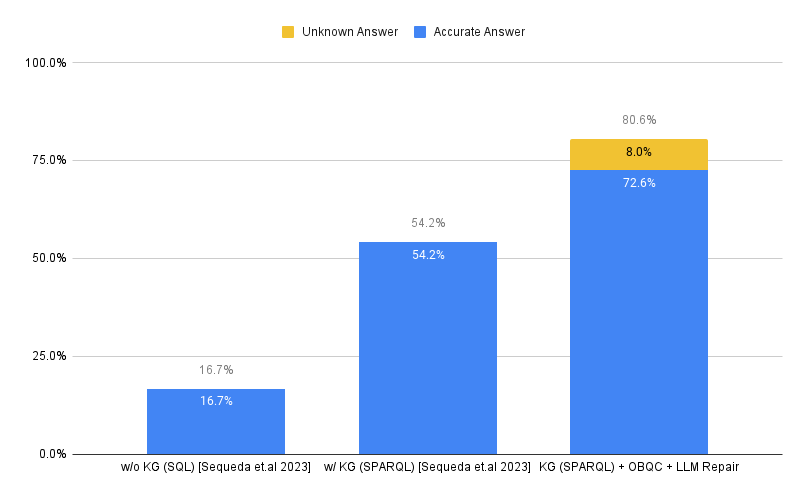
\includegraphics[scale=0.5]{submissions/Juan2024/results/OverallResultsWithPrevious.png}
\caption{Average Overall Execution Accuracy (AOEA) of SPARQL and SQL for all the questions in the benchmark compared to OBQC and LLM Repair}
\label{fig:OverallResultsWithPrevious}
\end{figure}

\begin{figure}[hbtp]
\centering
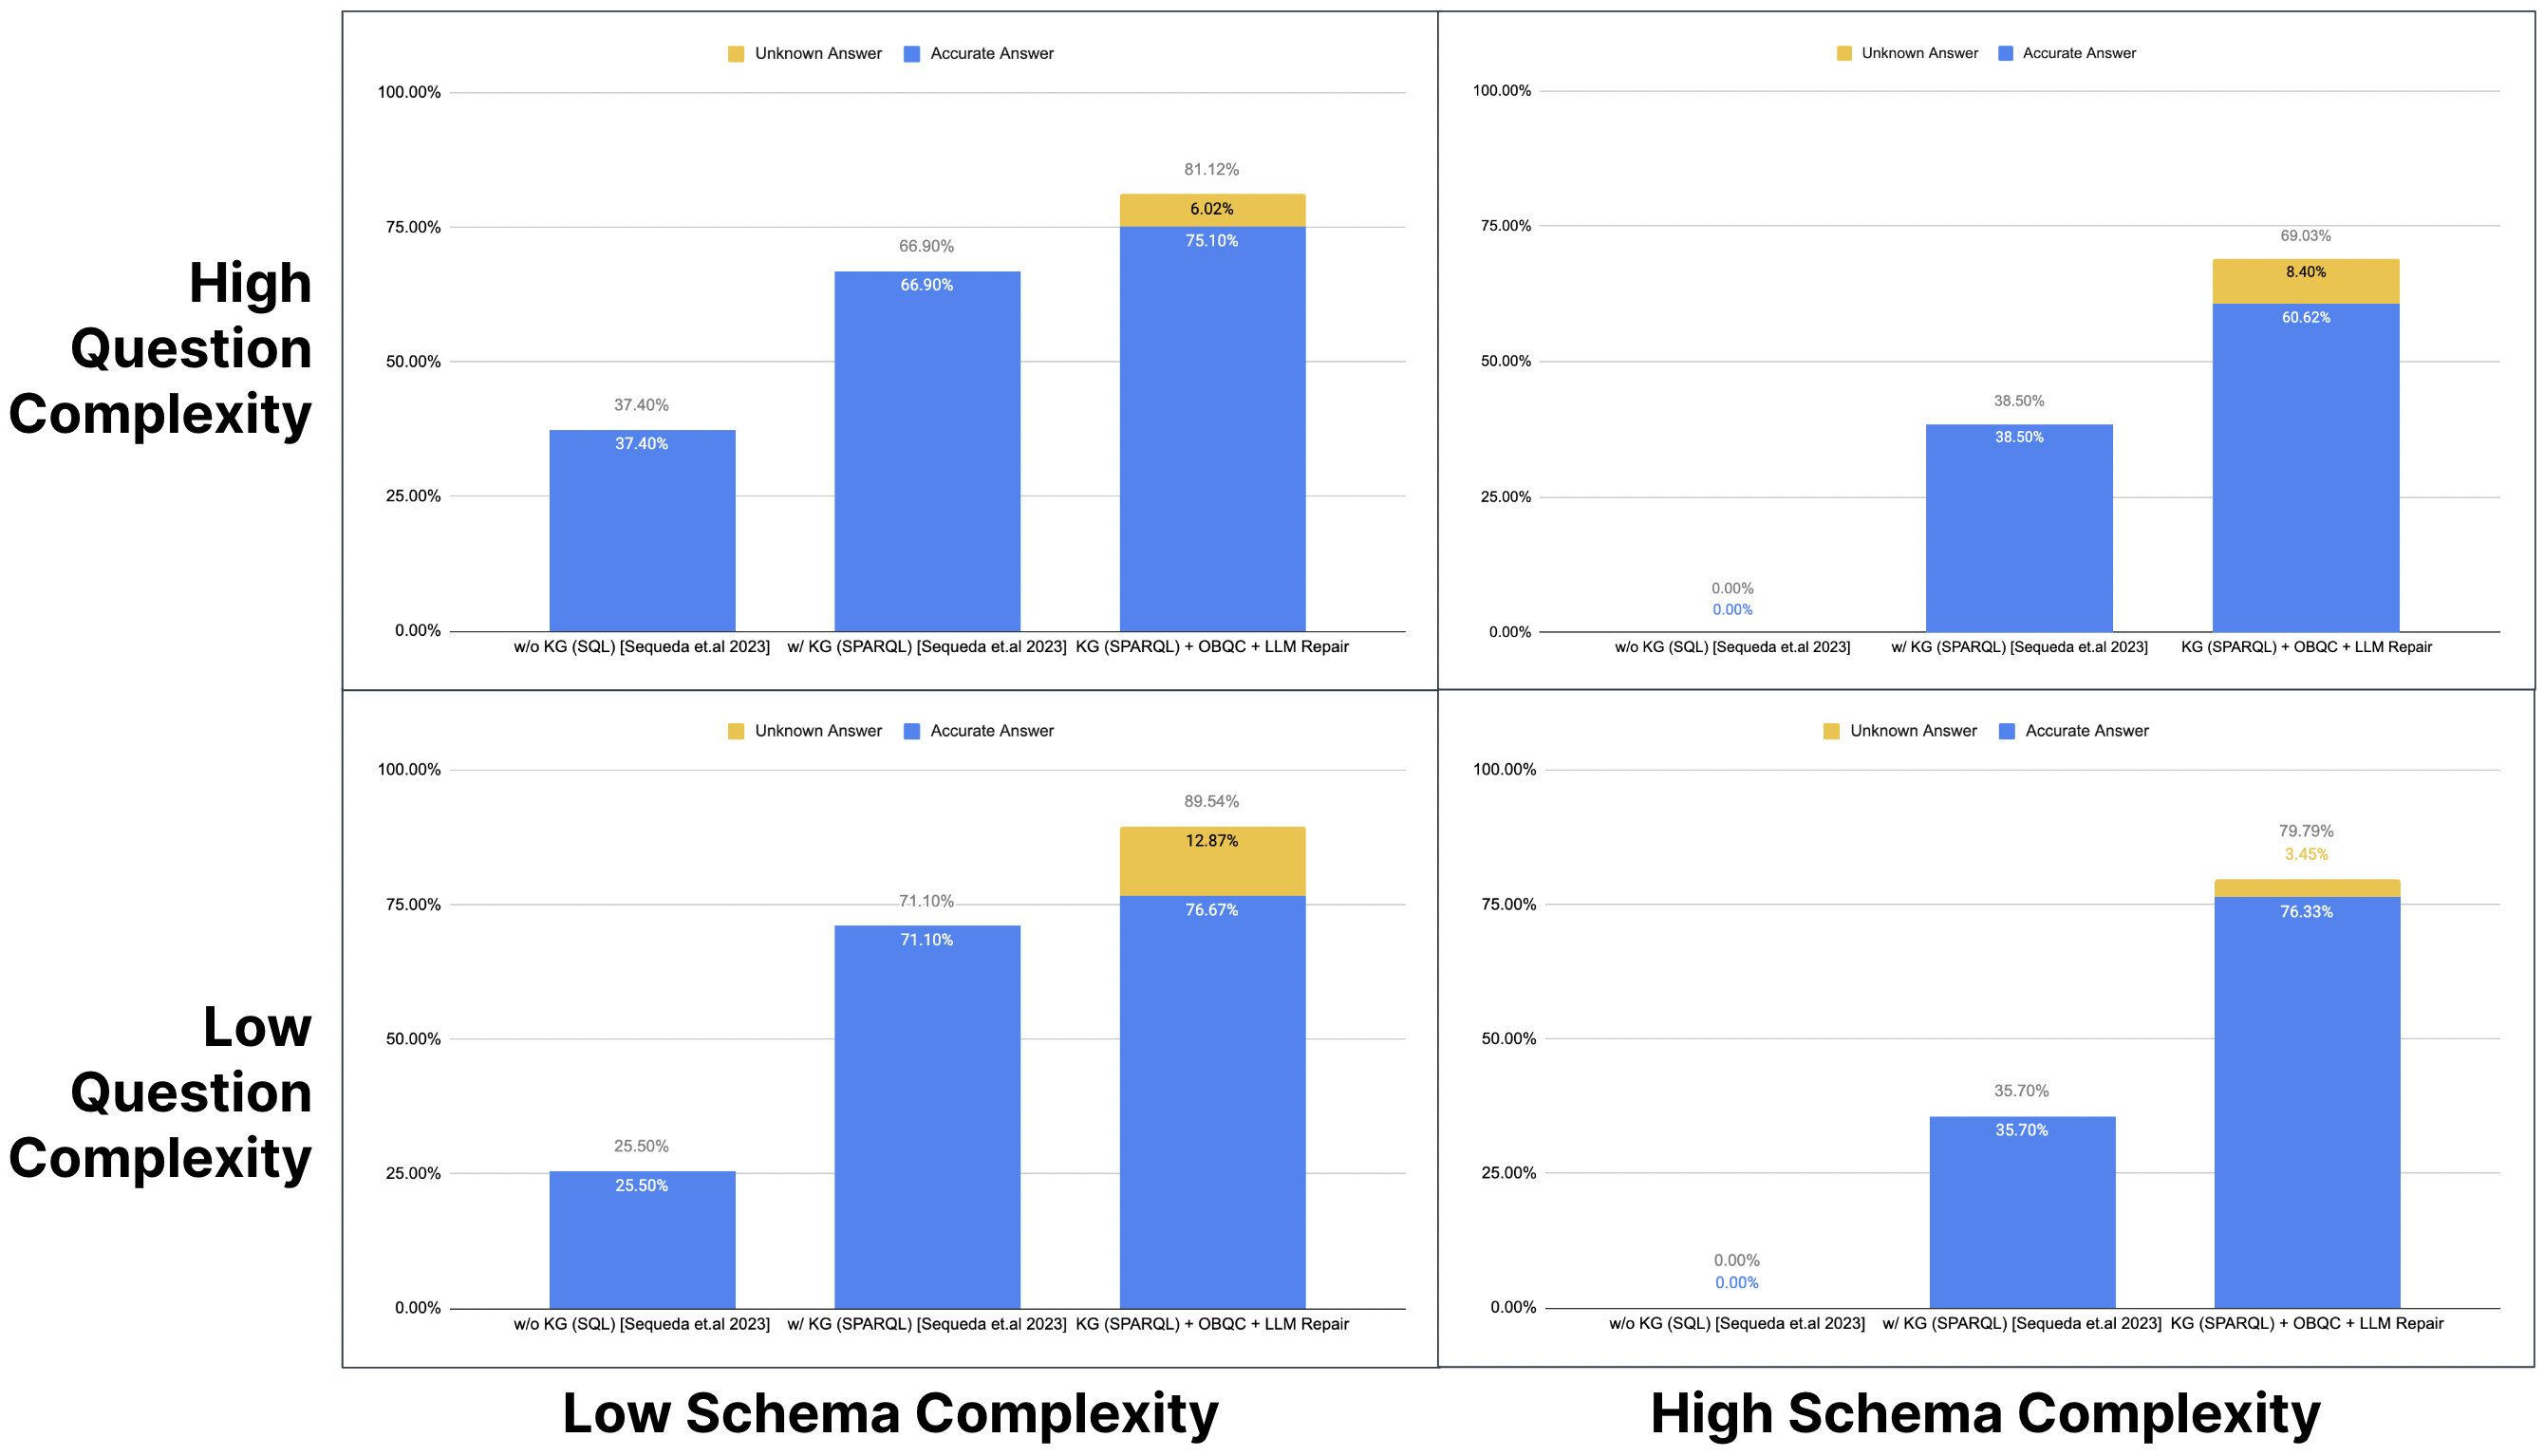
\includegraphics[scale=0.35]{submissions/Juan2024/results/QuadrantResultsWithPrevious.png}
\caption{Average Overall Execution Accuracy (AOEA) of SPARQL and SQL for all questions in each quadrant compared to OBQC and LLM Repair}
\label{fig:QuadrantResultsWithPrevious}
\end{figure}

%These results are evidence that supports our hypothesis, ontologies can further improve the accuracy of LLM powered question answering systems.

A follow up question to understand the \textit{extent} is the following: 
\textit{How much of the possible execution accuracy improvement was achieved?}
In other words, given the number of times the system achieved an accurate answer on the first time, and the total number of runs, we know how much is left for improvement. Therefore, how much of that improvement was achieved? 
For example, given a total of 10 runs, where 2 of them were accurate on the first try achieving a First Time Execution Accuracy of 20\%, means that there are 8 runs left where the OBQC and LLM Repair to repair a query in order to achieve 100\% Execution Accuracy with Repairs. Let's say that the system is able to accurately repair 4 times, therefore the Execution Accuracy with Repairs is 60\%. 
The achievable improvement is 50\% because the accurate repair occurred 4 times out of the 8 possible times. 
Achievable Improvement is calculated as (Number of Accurately Repaired Queries) / (Total Number of runs - Number of First Time Executed Accurate queries).
The results of achievable improvement are shown in Table \ref{table:AchievableImprovementResults}

%\begin{table}[h!]
\begin{wraptable}{r}{0.5\textwidth}
\centering
\begin{tabular}{ | m{5cm} | m{3cm} |} 
\hline
  & \textbf{Average Achievable Improvement}\\ 
  \hline
  \textbf{All Questions}   & 55.57\% \\ 
  \hline
  \textbf{Low Question/Low Schema}& 49.30\% \\ 
  \hline
  \textbf{High Question/Low Schema}& 40.45\% \\ 
  \hline
  \textbf{Low Question/High Schema}& 72.23\% \\  
  \hline
  \textbf{High Question/High Schema}& 57.70\% \\ 
  \hline
\end{tabular}
\caption{Average Achievable Improvement of Overall and Quadrant Results}
\label{table:AchievableImprovementResults}
%\end{table}
\end{wraptable}

The results indicate that the OBQC is able to successfully repair queries half of the time. 
Thus, we are halfway there and there is still room for improvement. 
Recall that OBQC mainly checks the body of the query and just two checks in the SELECT clause determine if IRI identifiers are returned. 
We postulate that a set of inaccurate queries are due to the overlap type of partial accurate queries: the columns returned by the query are correct, however, they are a subset of the accurate answer.
Therefore possible repair rules can be defined to check the head of the query.
Additionally, this may indicate the need for more expressive ontologies. 

\subsubsection{Error Type Results}

In our experiments, we kept count of the number of times a rule was invoked by the OBQC.
Table \ref{table:RuleUsage} presents the percentage of usage of each rule in the OBQC. 
Notably, 70\% of the repairs were done by the Body rules checks while 30\% of the repairs were done by the Head rules. 
The rules exclusively related to domain were invoked 42.16\% of the time and surprisingly, rules exclusively related to range were invoked less than 1\% of the time. 
The Domain Range rule contributed to 22.78\% of the repairs.

%\begin{table}[h!]
\begin{wraptable}{r}{0.5\textwidth}
\centering
\begin{tabular}{ | m{3cm} | m{2cm} |} 
\hline
  \textbf{Rule} & \textbf{Usage}\\ 
  \hline
  Double Domain   & 37.47\% \\ 
  \hline
  Domain Range   & 22.78\% \\ 
  \hline
  IRI Output& 18.40\% \\ 
  \hline
  Subject Output& 11.91\% \\  
  \hline
  Domain& 4.69\% \\ 
  \hline
  Incorrect Property& 4.26\% \\ 
  \hline
  Range& 0.43\% \\ 
  \hline
  Double Range& 0.06\% \\ 
  \hline
\end{tabular}
\caption{Rule usage in the Ontology-based Query Check}
\label{table:RuleUsage}
%\end{table}
% \vspace{-2cm}
\end{wraptable}

A surprising result is that the domain related rules had the largest impact in repairs. 
These results may shine some light on what is happening underneath the hood inside an LLM, namely the relationship between english language and triples of a graph. 
English is written and read from left to right. 
The domain of a property has a relationship to the left side of a triple.
If the LLM writes a query which is wrong, it would most probably get it wrong at the beginning of a sentence/triple. 
This may be an explanation on why the domain related rules were the most impactful. 

\section{Conclusion}
We are now able to provide answers to our research questions:

\noindent\textbf{RQ1:} To what extent Large Language Models (LLMs) can accurately answer Enterprise Natural Language questions over Enterprise SQL databases. 

\textbf{Answer:} Using GPT-4 and zero-shot prompting, Enterprise Natural Language questions over Enterprise SQL databases achieved 16.7\% Average Overall Execution Accuracy. For Low Question/Low Schema, the Overall Execution Accuracy was 25.5\%. For High Question/Low Schema, the Overall Execution Accuracy was 37.\%. However, for both Low Question/High Schema and High Question/High Schema, the accuracy was 0\%.

\noindent\textbf{RQ2:} To what extent Knowledge Graphs can improve the accuracy of Large Language Models (LLMs) to answer Enterprise Natural Language questions over Enterprise SQL databases. 

\textbf{Answer:} Using GPT-4 and zero-shot prompting, Enterprise Natural Language question over a Knowledge Graph representation of the enterprise SQL database achieved 54.2\% Average Overall Execution Accuracy. 
The overall SPARQL accuracy was 3x the SQL accuracy and the accuracy improvement was 37.5\%. 
% For Low Question/Low Schema, the Overall Execution Accuracy was 71.1\%, which is 2.8X the SQL accuracy and 45.6\% accuracy improvement. 
% For High Question/Low Schema, the Overall Execution Accuracy was 66.9\%, which is 1.8X the SQL accuracy and 29.5\% accuracy improvement. 
% For Low Question/High Schema, the Overall Execution Accuracy was 35.7\% and the improvement was also 35.7\%. 
% For High Question/High Schema, the Overall Execution Accuracy was 38.7\% and the improvement was also 38.7\%.

% One can argue that this was a predictable result given that the SPARQL query over a Knowledge Graph representation of the SQL database contains all the required context. 
% However, recall that these two research question is to understand \textit{to what extent} Large Language Models (LLMs) can accurately answer Enterprise Natural Language questions over Enterprise SQL databases and how much that extent increases by using Knowledge Graphs. 
% To the best of our knowledge, this extent was not understood until now. 

\noindent\textbf{RQ3}: To what extent can the accuracy increase by leveraging the ontology of a knowledge graph to detect errors of a SPARQL query and an LLM to repair the errors?

\textbf{Answer:} By using the same zero-shot prompting on GPT-4 and adding the Ontology-Based Query Check and LLM Repair, that new accuracy is 72.55\%.
That is over a 4x accuracy improvement compared to the zero-shot promting with SQL. 
% If we look at the error rate, we also see a substantial decrease. 
% Without leveraging a knowledge graph, the error rate is 83.3\%.
% % The error rate decreased to 45.8\% when using a knowledge graph.
Given that we consider an unknown result in our approach because the LLM Repair is not able to repair and the Ontology-Based Query Check catches the error, the overall error rate is 19.44\%. 

    
\noindent\textbf{RQ4}: What types of errors are most commonly presented in SPARQL queries generated by an LLM?

\textbf{Answer:} 70\% of the repairs were done by the Ontological checks while 30\% of the repairs were done by the SELECT Clause checks. 
The domain related rules had the largest impact in repairs, being invoked 42.16\% of the time. 
An interpretation of this result is that if the LLM writes a query which is wrong, it would most probably get it wrong at the beginning of a sentence/triple and the domain of a property has a relationship to the left side of a triple.

The answers to our research questions are evidence that supports the main conclusion of our work: Knowledge Graph provides higher accuracy for LLM powered question answering systems on SQL databases.

What is evident is that context is crucial for accuracy and these results further emphasizes the need to invest in business context. 
The point to be made here is a call to action that investing in context of SQL databases is required to increase the accuracy of LLMs for question answering over the SQL databases. 
In this work, the context was presented in the form of a knowledge graph consisting of an ontology that describes the semantics of the business domain and mappings that connect the physical schema with the ontology which are used to create the knowledge graph. 
The ontology can also include further semantics such as synonyms, labels in different languages, which are not expressible in a SQL DDL. 

Arguably, our work has influenced the wider data industry to acknowledge the need to invest in semantics and knowledge graphs in this new AI era. 
Our work has been reproduced and validated by multiple independent vendors\footnote{https://roundup.getdbt.com/p/semantic-layer-as-the-data-interface}\footnote{https://www.atscale.com/blog/semantic-layers-make-genai-more-accurate/}
\footnote{https://www.wisecube.ai/blog/optimizing-llm-precision-with-knowledge-graph-based-natural-language-qa-systems/}
\footnote{https://blog.kuzudb.com/post/llms-graphs-part-1/}
\footnote{https://delphihq.substack.com/p/delphi-at-100-dbt-semantic-layer}
\footnote{https://cube.dev/blog/semantic-layers-the-missing-piece-for-ai-enabled-analytics}
\footnote{https://www.stratio.com/blog/stratio-business-semantic-data-layer-delivers-99-answer-accuracy-for-llms/}, and contributed to rise of GraphRAG\footnote{https://neo4j.com/blog/graphrag-manifesto/}.

The takeaway for enterprises is that in order to provide trustworthy question answering systems that results in highly accurate results, they must make an investment in business context and semantics. This context needs to be effectively managed in metadata managements systems such as data catalog and governance platforms built on a knowledge graph architecture. 



\bibliographystyle{plain}
\bibliography{references}



\end{document}
